%% LyX 2.1.0 created this file.  For more info, see http://www.lyx.org/.
%% Do not edit unless you really know what you are doing.
\documentclass[english]{article}
\usepackage[T1]{fontenc}
\usepackage[latin9]{inputenc}
\usepackage{color}
\usepackage{verbatim}
\usepackage{amsthm}
\usepackage{amsmath}
\usepackage{amssymb}
\usepackage{graphicx}
\usepackage{esint}

\makeatletter
%%%%%%%%%%%%%%%%%%%%%%%%%%%%%% Textclass specific LaTeX commands.
\theoremstyle{plain}
\newtheorem{thm}{\protect\theoremname}
  \theoremstyle{plain}
  \newtheorem{lem}[thm]{\protect\lemmaname}

%%%%%%%%%%%%%%%%%%%%%%%%%%%%%% User specified LaTeX commands.
% UAI 2015 template
\usepackage{proceed2e}

\usepackage{algorithmic}
\usepackage{algorithm}

\renewcommand{\algorithmicrequire}{\textbf{Input:}}
\renewcommand{\algorithmicensure}{\textbf{Output:}}

\usepackage{appendix}
\usepackage{amsmath}
\usepackage{amsfonts}
\usepackage{amsthm}
\usepackage{enumerate}
%\usepackage{etex}

    \usepackage[ plainpages = true, pdfpagelabels, 
                 pdfpagelayout = useoutlines,
                 bookmarks,
                 bookmarksopen = true,
                 bookmarksnumbered = true,
                 breaklinks = true,
                 linktocpage,
                 pagebackref,
                 colorlinks = true,
                 linkcolor = blue,
                 urlcolor  = blue,
                 citecolor = blue!50!black,
                 anchorcolor = green,
                 hyperindex = true,
                 hyperfigures
                 ]{hyperref} 
%\usepackage{index}
%\usepackage{longtable}

%\usepackage{mdwlist}
\usepackage{natbib}
\usepackage[resetlabels,labeled]{multibib}
%\usepackage{microtype}
\usepackage{soul}
\usepackage{subfig}
\usepackage{tikz}
\usepackage[textsize=small]{todonotes}

\usepackage{url}
%\usepackage[all]{xy}

%\usepackage{epstopdf}
%\usepackage{auto-pst-pdf}



\newcommand{\diag}{\mathop{\mathrm{diag}}}
\newcommand{\trace}{\mathop{\mathrm{tr}}}
\newcommand{\median}{\mathop{\mathrm{median}}}

\newcommand{\wjnote}[1]{\textbf{\color{blue!80!black}{WJ: #1}} }
\newcommand{\aenote}[1]{\textbf{\color{red!50!black}{#1}} }
\newcommand{\nhnote}[1]{\textbf{\color{magenta!90!black}{#1}} }
\newcommand{\agnote}[1]{\textbf{\color{green!50!black}{#1}} }

\newcommand{\figref}[1]{Fig.~\ref{#1}}
\newcommand{\secref}[1]{Sec.~\ref{#1}}
\newcommand{\tabref}[1]{Table.~\ref{#1}}
%\newcommand{\eqref}[1]{Eq.~\ref{#1}}

\newcites{sup}{Supplementary}

\makeatother

\usepackage{babel}
  \providecommand{\lemmaname}{Lemma}
\providecommand{\theoremname}{Theorem}

\begin{document}

\title{Kernel-Based Just-In-Time Learning for Passing Expectation Propagation
Messages}
\author{}

\maketitle
\begin{abstract}
We propose to learn a kernel-based message operator which takes as input all
expectation propagation (EP) incoming messages to a factor node and
produces an outgoing message. In ordinary EP, computing an outgoing
message involves estimating a multivariate integral which may not
have an analytic expression. Learning such an operator allows one
to bypass the expensive computation of the integral during inference
by directly mapping all incoming messages into an outgoing message.
The operator can be learned online during inference (from examples of input
and output messages) which allows automated inference to be made on
any kind of factor that can be sampled.
\aenote{AE: 1. State the problem. 2. Say why it's interesting. 3. Say what your solution achieves. 4. Say what follows from your solution. Message-passing is useful. Message-passing in general is slow. Our approach speeds it up. This allows us to use it on more complicated / larger problems.}
\end{abstract}

\section{Introduction}
In \verb|kernel_ep_uai2015_v2.tex| Nicolas and Ali have a new introduction.

\section{Background}
\wjnote{Do we need both introduction and background sections ?}

Existing approaches to automated probabilistic inference can be broadly
divided into two categories \citep{Heess2013}: uninformed and informed
cases. In the uninformed case, the modeler has full freedom in expressing
a probabilistic model without any constraint on the set of usable
factors. This high flexibility comes at a price during inference as
less factor-specific information is available to the inference engine.
Often MCMC-based sampling techniques are employed by treating the
factors as black boxes. In the informed case \citep{SDT2014,Minka2012},
the modeler is required to build a model from constructs whose necessary
computations are known to the inference engine. Although efficient
during the inference, using an unsupported construct would require
manual derivation and implementation of the relevant computations
in the inference engine. 

In this work, we focus on EP, a commonly used approximate inference
method. Following \cite{Heess2013, Eslami2014}, we propose to learn a kernel-based
message operator for EP to capture the relationship between incoming
messagesj to a factor and outgoing messages. The operator bridges
the gap between the uninformed and informed cases by automatically
deriving the relevant computations for any custom factor that can
be sampled. This hybrid approach gives the modeler as much flexibility
as in the uninformed case while offering efficient message updates
as in the informed case. This approach supports fast inference as
no expensive KL divergence minimization needs to be done during inference
as in ordinary EP. In addition, a learned operator for a factor is
reusable in other models in which the factor appears. As will be seen,
to send an outgoing message with the kernel-based operator, it is
sufficient to generate a feature vector for incoming messages and
multiply with a pre-learned matrix. Unlike \cite{Heess2013} which
considers a neural network, the kernel-based message operator we propose
can be easily extended to allow online updates of the operator during
inference. 

\wjnote{add some text to link to ridge regression. Then...}
By virtue of the primal form, it is straightforward to derive an update
equation for an online-active learning during EP inference: if the
predictive variance  on the current incoming messages is high, then we query the outgoing message from
the importance sampler (oracle) and update the operator. Otherwise,
the outgoing message is efficiently computed by the operator. Online
learning of the operator lessens the need of the distribution on natural
parameters of incoming messages used in training set generation. Determining
an appropriate distribution was one of the unsolved problems in \cite{Heess2013}. 

\hl{TODO/TO add:}
\begin{itemize}
\item Mention that online learning improves Nicolas's batch training approach. 
\item To connect to Ali's work, can mention that online learning of random
forests is difficult. Online learning is straightforward and exact
for Bayesian linear regression. May ask Balaji more on relevant citations.
\item It was argued in \cite{Hutter2009} (Section 11.2) that a random forest
may have problems with exploring previously-unseen areas of the input
domain.
\end{itemize}
\hrule{}

\begin{comment}
Below we give a short introduction to EP in Sec. \ref{sec:Expectation-Propagation-(EP)},
and propose the kernel-based operator in Sec. \ref{sec:Learning-to-Pass}.
A proof-of-concept experiment on the operator is given in Sec. \ref{sec:Experiments}.
Finally, we conclude with remarks on future directions in Sec. \ref{sec:Conclusions-and-Future}.
\end{comment}


\begin{comment}
\begin{itemize}
\item the need for automated inference. => learning a message operator to
send an outgoing message given incoming messages.
\item reusable, online update. Potential use in a probabilistic programming
language (PPL). 
\item Talk about a few PPLs. Talk about their approaches which are mostly
sampling. Drawback of sampling ?
\item Focus on EP here. A few comments on EP advantage ?
\end{itemize}
Split the conventional inference into 2 stages: training of a message
operator and actual inference.

Merits:

\textbf{Support fast inference. }No need to minimize multidimensional
KL divergence during actual inference. To send a message, compute
matrix $\times$ vector. \textbf{Automated inference}. No need to
derive complex message updates. \textbf{Applicable to any complex
factor. }Only requirement = ability to sample from the factor. No
need to be able to evaluate the likelihood value. Potential use in
a probabilistic programming language.\textbf{ Operator reusable }once
trained.
\end{comment}



\section{Expectation Propagation (EP)\label{sec:Expectation-Propagation-(EP)}}

Expectation propagation \citep{Minka2001,Bishop2006} (EP) is a commonly
used approximate inference method for inferring the posterior distribution
of latent variables given observations. In a typical directed graphical
model, the joint distribution of the data $X=\left\{ X_{1},\ldots,X_{n}\right\} $
and latent variables $\theta=\left\{ \theta_{1},\ldots,\theta_{t}\right\} $
takes the form of a product of factors, $p(X,\theta)=\prod_{i=1}^{m}f_{i}(X|\theta)$
where each factor $f_{i}$ may depend on only a subset of $X$ and
$\theta$. With $X$ observed, EP approximates the posterior with
$q(\theta)\propto\prod_{i=1}^{m}m_{f_{i}\rightarrow\theta}(\theta)$
where $m_{f_{i}\rightarrow\theta}$ is an approximate factor corresponding
to $f_{i}$ with the constraint that it has a chosen parametric form
(e.g., Gaussian) in the exponential family (ExpFam). EP takes into
account the fact that the final quantity of interest is the posterior
$q(\theta)$ which is given by the product of all approximate factors.
In finding the $i^{th}$ approximate factor $m_{f_{i}\rightarrow\theta}$,
EP uses other approximate factors $m_{\theta\rightarrow f_{i}}(\theta):=\prod_{j\neq i}m_{f_{j}\rightarrow\theta}(\theta)$
as a context to determine the plausible range of $\theta$. EP iteratively
refines $m_{f_{i}\rightarrow\theta}$ for each $i$ with \wjnote{No need to mention this special-case msg.}$m_{f_{i}\rightarrow\theta}(\theta)=\frac{\text{proj}\left[\int dX\, f(X|\theta)m_{X\rightarrow f_{i}}(X)m_{\theta\rightarrow f_{i}}(\theta)\right]}{m_{\theta\rightarrow f_{i}}(\theta)}$
where $\text{proj}\left[r\right]=\arg\min_{q\in\text{ExpFam}}\text{KL}\left[r\,\|\, q\right]$
and $m_{X\rightarrow f_{i}}(X):=\delta(X-X_{0})$ if $X$ is observed
to be $X_{0}$. In the EP literature, $m_{\theta\rightarrow f_{i}}$
is known as a cavity distribution. \aenote{AE: Too many inline equations.} 

The projection can be carried out by the following moment matching
procedure. Assume an ExpFam distribution $q(\theta|\eta)=h(\theta)\exp\left(\eta^{\top}u(\theta)-A(\eta)\right)$
where $u(\theta)$ is the sufficient statistic\textbf{ }of $q$, $\eta$
is the natural parameter and $A(\eta)=\log\int d\theta\, h(\theta)\exp\left(\eta^{\top}u(\theta)\right)$
is the log-partition function. It can be shown that $q^{*}=\text{proj}\left[r\right]$
satisfies $\mathbb{E}_{q^{*}(\theta)}\left[u(\theta)\right]=\mathbb{E}_{r(\theta)}\left[u(\theta)\right].$
That is, the projection of $r$ onto ExpFam is given by $q^{*}\in\text{ExpFam}$
that has the same moment parameters as the moments under $r$. 

\wjnote{Should jump to this general msg from the beginning.}In general,
under the approximation that each factor fully factorizes, an EP message
from a factor $f$ to a variable $V$ takes the form 
\begin{align}
m_{f\rightarrow V}(v) & =\frac{\text{proj}\left[\int d\mathcal{V}\backslash\{v\}\, f(\mathcal{V})\prod_{V'\in\mathcal{V}}m_{V'\rightarrow f}(v')\right]}{m_{V\rightarrow f}(v)}\nonumber \\
 & :=\frac{\text{proj}\left[r_{f\rightarrow V}(v)\right]}{m_{V\rightarrow f}(v)}:=\frac{q_{f\rightarrow V}(v)}{m_{V\rightarrow f}(v)}\label{eq:general_ep_msg}
\end{align}
where $\mathcal{V}=\mathcal{V}(f)$ is the set of variables connected
to $f$ in the factor graph. In the previous case of $m_{f_{i}\rightarrow\theta}$,
we have $\mathcal{V}(f)=\left\{ X,\theta\right\} $ and $V$ in Eq.
\ref{eq:general_ep_msg} corresponds to $\theta$. Typically, when
the factor $f$ is complicated, the integral defining $r_{f\rightarrow V}$
becomes intractable. Quadrature rules or other numerical integration
techniques are often applied to approximate the integral. \aenote{AE: This is the main point we want to get accross. Either needs more emphasis or should be mentioned sooner.}


\section{Learning to Pass EP Messages\label{sec:Learning-to-Pass}}

Our goal is to learn a message operator $C_{f\rightarrow V'}$ with
signature $\left[m_{V\rightarrow f}\right]_{V\in\mathcal{V}(f)}\mapsto q_{f\rightarrow V'}$
which takes in all incoming messages $\left\{ m_{V\rightarrow f}\mid V\in\mathcal{V}(f)\right\} $
and outputs $q_{f\rightarrow V'}(v')$ i.e., the numerator of Eq.
\ref{eq:general_ep_msg}. For inference, we require one such operator
for each recipient variable $V'\in\mathcal{V}(f)$ i.e., in total
$|\mathcal{V}(f)|$ operators need to be learned for $f$. Operator
learning is cast as a distribution-to-distribution regression problem
where the training set $S_{V'}:=\{([m_{V\rightarrow f}^{n}]_{V\in\mathcal{V}(f)},q_{f\rightarrow V'}^{n})\}_{n=1}^{N}$containing
$N$ incoming-outgoing message pairs can be generated as in \cite{Heess2013,Eslami2014}
by importance sampling to compute the mean parameters $\mathbb{E}_{r_{f\rightarrow V'}(v')}\left[u(v')\right]$
for moment matching. In principle, the importance sampling itself
can be used in EP for computing outgoing messages \citep{Barthelme2011}.
The scheme is, however, expensive as we need to draw a large number
of samples for each outgoing message to be sent. In our case, the
importance sampling is used for data set generation which is done
offline before the actual inference.

The assumptions needed for the generation of a training set are as
follows. First, we assume the factor $f$ takes the form of a
conditional distribution $f(v_{1}|v_{2},\ldots,v_{|\mathcal{V}(f)|})$.
Second, given $v_{2},\ldots,v_{|\mathcal{V}(f)|}$, $v_{1}$ can
be sampled from $f(\cdot|v_{2},\ldots,v_{|\mathcal{V}(f)|})$. 
The ability to evaluate $f$ is not assumed. 
In contrast to \cite{Heess2013}, we do not assume that a distribution on the natural parameters of all incoming messages is available. \wjnote{because we use onlne-active learning... More text here.}

%Finally we assume that a distribution on the natural parameters of all incoming messages $\left\{ m_{V\rightarrow f}\right\} _{V\in\mathcal{V}(f)}$
%is available. The distribution is used solely to give a rough idea
%of incoming messages the learned operator will encounter during the
%actual EP inference. In practice, we only need to ensure that the
%distribution sufficiently covers the relevant region in the space
%of incoming messages. 
%\aenote{AE: This sentence needs reworking now that you only train on messages observed in the model.}

In recent years, there have been a number of works on the regression
task with distributional inputs, including \cite{Poczos2013,Szabo2014}
which mainly focus on the non-parametric case and are operated under
the assumption that the samples from the distributions are observed
but not the distributions themselves. In our case, the distributions
(messages) are directly observed. Moreover, since the distributions
are in ExpFam, they can be characterized by a finite-dimensional natural
parameter vector or expected sufficient statistic. Hence, we can simplify
our task to distribution-to-vector regression where the output vector
contains a finite number of moments sufficient to characterize $q_{f\rightarrow V'}$.
As regression input distributions are in ExpFam, one can also treat
the task as vector-to-vector regression. However, seeing the inputs
as distributions allows one to use kernels on distributions which
are invariant to parametrization.


\section{Proposed Method}

In principle, any distribution-to-vector regression function can be applied to learn a message operator $C_{f\rightarrow V'}$, once the training set $S_{V'}$ is obtained.
Given incoming messages, the operator outputs $q_{f\rightarrow V'}$
from which the outgoing EP message is given by $m_{f\rightarrow V'}=q_{f\rightarrow V'}/m_{V'\rightarrow f}$
which can be computed analytically. We opt for kernel ridge regression
\citep{Scholkopf2002} as our message operator for its simplicity,
its ease of use in an online setting during inference (see \secref{sec:kernel_ep_online}), and rich supporting theory. 

\subsection{Kernel Ridge Regression}
\wjnote{We need to unify Kernel ridge regression and Bayesian linear regression sections. 
Posterior mean estimate of the Bayesian regression is the same as the solution to primal kernel ridge regression.
Bayesian regression assumes a Gaussian noise output allowing us to compute predictive variance.}


%\aenote{AE: Too many inline equations in this section. Pull out the most important ones?} 
We consider here the problem of regressing smoothly from distribution-valued
inputs to feature-valued outputs. We follow the regression framework
of \cite{Micchelli2005}, with convergence guarantees provided by
\cite{Caponnetto2007}. Under smoothness constraints, this regression
can be interpreted as computing the conditional expectation of the
output features given the inputs \citep{Gruenewaelder2012}.

Let $\mathsf{X}=\left(\mathsf{x}_{1}|\cdots|\mathsf{x}_{N}\right)$
be the training regression inputs and $\mathsf{Y}=\left(\mathbb{E}_{q_{f\rightarrow V'}^{1}}u(v')|\cdots|\mathbb{E}_{q_{f\rightarrow V'}^{N}}u(v')\right)\in\mathbb{R}^{D_{y}\times N}$
be the regression outputs. The ridge regression in the primal form
seeks $\mathsf{W}\in\mathbb{R}^{D_{y}\times D}$ for the regression
function $g(\mathsf{x})=\mathsf{W}\mathsf{x}$ which minimizes the
squared-loss function $J(\mathsf{W})=\sum_{i=1}^{N}\|\mathsf{y}_{i}-\mathsf{W}\mathsf{x}_{i}\|_{2}^{2}+\lambda\trace\left(\mathsf{W}\mathsf{W}^{\top}\right)$
where $\lambda$ is a regularization parameter and $\trace$ denotes
a matrix trace. 

It is well known that the solution is given by $\mathsf{W}=\mathsf{Y}\mathsf{X}^{\top}\left(\mathsf{X}\mathsf{X}^{\top}+\lambda I\right)^{-1}$
which has an equivalent dual solution $\mathsf{W}=\mathsf{Y}\left(K+\lambda I\right)^{-1}\mathsf{X}^{\top}=A\mathsf{X}^{\top}$
. The dual formulation allows one to regress from any type of input
objects if a kernel can be defined between them. All the inputs enter to the regression
function through the gram matrix $K\in\mathbb{R}^{N\times N}$ where
$\left(K\right)_{ij}=\kappa(\mathsf{x}_{i},\mathsf{x}_{j})$ yielding
the regression function of the form $g(\mathsf{x})=\sum_{i=1}^{N}a_{i}\kappa(\mathsf{x}_{i},\mathsf{x})$
where $A:=(a_{1}|\cdots|a_{N})$. The dual formulation therefore allows
one to straightforwardly regress from incoming messages to vectors
of mean parameters.
Although this property is appealing, the training
size $N$ in our setting can be chosen to be arbitrarily large, making
computation of $g(\mathsf{x})$ expensive for a new unseen point $\mathsf{x}$.


To eliminate the dependency on $N$, we propose to apply random Fourier
features \citep{Rahimi2007} $\hat{\phi}(\mathsf{x})\in\mathbb{R}^{D}$
for $\mathsf{x}:=[m_{V\rightarrow f}]_{V\in\mathcal{V}(f)}$ such
that $\kappa(\mathsf{x},\mathsf{x}')\approx\hat{\phi}(\mathsf{x})^{\top}\hat{\phi}(\mathsf{x}')$
where $D$ is the number of random features. The use of the random
features allows us to go back to the primal form of which the regression
function $g(\hat{\phi}(\mathsf{x}))=\mathsf{W}\hat{\phi}(\mathsf{x})$
can be computed efficiently. In effect, computing an EP outgoing message
requires nothing more than a multiplication of a matrix $\mathsf{W}$
($D_{y}\times D$ ) with the $D$-dimensional feature vector generated
from the incoming messages. 


\subsection{Bayesian Linear Regression}

Denote $X=\left(x_{1}|\cdots|x_{N}\right)\in\mathbb{R}^{D\times N}$
as (finite-dimensional) input and $Y=\left(y_{1}|\cdots|y_{N}\right)\in\mathbb{R}^{1\times N}$
(one coordinate of all expected sufficient statistics) as regression
output. In our application, $x_{n}$ will denote a random feature
vector for $[m_{V\rightarrow f}^{n}]_{V\in\mathcal{V}(f)}$. Assume
%
\begin{align*}
w & \sim\mathcal{N}\left(w;0,I_{D}\sigma_{0}^{2}\right)\\
Y\mid X,w & \sim\mathcal{N}\left(Y;w^{\top}X,\sigma_{y}^{2}I_{N}\right).
\end{align*}
%
The output noise variance $\sigma_{y}^{2}$ should capture the intrinsic
stochasticity of the importance sampler used to generate $Y$. It
follows that the posterior of $w$ is given by \citep{Bishop2006}
\begin{align*}
p(w\mid Y) & =\mathcal{N}(w;\mu_{w},\Sigma_{w})\\
\Sigma_{w} & = \left( XX^{\top}\sigma_{y}^{-2}+\sigma_{0}^{-2}I \right)^{-1} \\
\mu_{w} & =\Sigma_{w}XY^{\top}\sigma_{y}^{-2}.
%=\left(XX^{\top}+\frac{\sigma_{y}^{2}}{\sigma_{0}^{2}}I\right)^{-1}XY^{\top}.
\end{align*}
The noise variance $\sigma_{y}^{2}$ is proportional to the regularization
parameter in linear regression. 
The predictive distribution on the output $y^{*}$ given an observation $x^{*}$ is
%
\begin{align*}
p(y^{*}|x^{*},Y) & =\int dw\, p(y^{*}|w,x^{*},Y)p(w|Y)\\
 & =\mathcal{N}\left(y^{*};x^{*\top}\mu_{w},x^{*\top}\Sigma_{w}x^{*}+\sigma_{y}^{2}\right)
% & =\mathcal{N}(y^{*};m^{*},v^{*}).
\end{align*}

% The marginal likelihood is given by
%\begin{align*}
%p(Y|X) & =\int dw\, p(Y|X,w)p(w)\\
% & =\mathcal{\mathcal{N}}\left(Y;0,K\sigma_{0}^{2}+\sigma_{y}^{2}I_{N}\right)\\
% & =\det\left(2\pi\Sigma\right)^{-1/2}\exp\left(-\frac{1}{2}Y^{\top}\left(K\sigma_{0}^{2}+\sigma_{y}^{2}I_{N}\right)^{-1}Y\right)
%\end{align*}
%where $K=X^{\top}X$ is a gram matrix of $X$. 
%One can do gradient ascent on $\log p(Y|X)$
%to optimize $\sigma_{0}^{2},\sigma_{y}^{2}$ and kernel parameters.

For simplicity, we treat each output (expected sufficient statistic) as a separate regression problem. 
Treating all outputs jointly can be achieved with a multi-output kernel \citep{Alvarez2011}.

\subsection{Online Update \label{sec:kernel_ep_online}}
 
In this section, we consider an online update for $\Sigma_{w}$ and
$\mu_{w}$ when observations $X$ comes in stream. We will use $\cdot^{(n)}$
to denote a quantity constructed from $n$ samples. Recall that $\Sigma_{w}^{-1(N)}=XX^{\top}\sigma_{y}^{-2}+\sigma_{0}^{-2}I$.
The posterior covariance matrix at time $N+1$ can be written as 
\begin{align*}
\Sigma_{w}^{(N+1)} & =\left(XX^{\top}\sigma_{y}^{-2}+ \sigma_{0}^{-2}I  
 + x_{N+1}x_{N+1}^{\top}\sigma_{y}^{-2} \right)^{-1}\\
 & =\left(\Sigma_{w}^{-1(N)}+x_{N+1}x_{N+1}^{\top}\sigma_{y}^{-2}\right)^{-1}\\
 & =\Sigma_{w}^{(N)}-\frac{\Sigma_{w}^{(N)}x_{N+1}x_{N+1}^{\top}\Sigma_{w}^{(N)}\sigma_{y}^{-2}}{1+x_{N+1}^{\top}\Sigma_{w}^{(N)}x_{N+1}\sigma_{y}^{-2}}
\end{align*}
where we used the Sherman-Morrison formula. 
In this form, the posterior covariance at time $N+1$ can be expressed in terms of 
the covariance at time $N$.
%\[
%\left(A+uv^{\top}\right)^{-1}=A^{-1}-\frac{A^{-1}uv^{\top}A^{-1}}{1+v^{\top}A^{-1}u}
%\]
%with $A=\Sigma_{w}^{-1(N)}$. 
Updating $\Sigma_{w}$ costs $O(D^{2})$ per one new observation. 
For $\mu_{w}=\Sigma_{w}XY^{\top}\sigma_{y}^{-2}$, we maintain
$XY^{\top}\in\mathbb{R}^{D}$ and update it with
\[
\left(XY^{\top}\right)^{(N+1)}=\left(XY^{\top}+x_{N+1}y_{N+1}\right), 
\]
costing $O(D)$ per update. 
%In the first iteration when no data are observed, $\Sigma_{w}^{(1)}=\sigma_{0}^{2}I$.

\wjnote{Mention initial minibatch training here.}

\subsection{Online-Active Learning}

%If the predictive variance of the current incoming messages $x^{*}$
%is high, the operator queries the correct outgoing message from the importance sampler
%(oracle) and update the $\Sigma_{w}$ and $\mu_{w}$. 
%Otherwise, the outgoing message is efficiently computed by the operator. 

Since we have $D_{y}$ regression functions, 
for each tuple of incoming messages $x^{*}$, there are $D_{y}$
predictive variances, $v_{1}^{*},\ldots,v_{D_{y}}^{*}$, one for each
output. 
Let $\{\tau_{i}\}_{i=1}^{D_{y}}$ be pre-specified predictive variance thresholds.
\wjnote{How should we choose these thresholds ?}
Given a new input $x^{*}$, if $v_{1}^{*}>\tau_{1}$ or $\cdots$
or $v_{D_{y}}^{*}>\tau_{D_{y}}$ i.e., the operator is uncertain, 
a query is made to the oracle to obtain a ground truth $y^{*}$. 
The pair $(x^{*},y^{*})$ is then
used to update $\Sigma_{w}$ and $\mu_{w}$ as described previously. 
%Querying the oracle incurs a high computational cost.


\subsection{Computational Complexity}
\wjnote{Compare ridge regression cost with Ali's forest here ?}

Let $K$ be the number of trees in the random forest,
$D$ be the dimensionality of message representation,
and $N$ be the number of oracle consultations so far.
Let $M$ be number of training points in each leaf.
Assuming that the depth of trees is $O(\log(N))$, one prediction from a random forest costs $O(KD\log(N))$, and one update costs $O(KD^2 \log(N))$.
This is because for each tree in forest $O(K)$, tree traversal takes $O(\log(N))$, 
and one prediction costs $O(D)$. 
One full training of a regression function costs $O(D^2 (D + M))$ which depends on $M$. 
However typically $M$ is negligible at a lower depth, a full training costs $O(D^3)$.
The total updating cost across all trees is $O(KD^3log(N))$.


\section{Kernels on Distributions}

A number of kernels on distributions have been studied in the literature
\citep{Jebara2003,Jebara2004}. Relevant to us are kernels whose random
features can be efficiently computed. Due to the space constraint,
we only give a few examples here.

\subsection{Expected Product Kernel}
An expected product kernel is also known as a set kernel. 
Let $\mu_{r^{(l)}}:=\mathbb{E}_{r^{(l)}(a)}k(\cdot,a)$ be the mean
embedding \citep{Smola2007} of the distribution $r^{(l)}$ into RKHS
$\mathcal{H}^{(l)}$ induced by the kernel $k$. Assume $k=k_{\text{gauss}}$
(Gaussian kernel) and assume there are $c$ incoming messages $\mathsf{x}:=(r^{(i)}(a^{(i)}))_{i=1}^{c}$
and $\mathsf{y}:=(s^{(i)}(b^{(i)}))_{i=1}^{c}$. The expected product
kernel $\kappa_{\text{pro}}$ is defined as 
\begin{align*}
\kappa_{\text{pro}}\left(\mathsf{x},\mathsf{y}\right) & :=\left\langle \bigotimes_{l=1}^{c}\mu_{r^{(l)}},\bigotimes_{l=1}^{c}\mu_{s^{(l)}}\right\rangle _{\otimes_{l}\mathcal{H}^{(l)}}\\
 & =\prod_{l=1}^{c}\mathbb{E}_{r^{(l)}(a)}\mathbb{E}_{s^{(l)}(b)}k_{\text{gauss}}^{(l)}\left(a,b\right)\approx\hat{\phi}(\mathsf{x})^{\top}\hat{\phi}(\mathsf{y})
\end{align*}
where $\hat{\phi}(\mathsf{x})^{\top}\hat{\phi}(\mathsf{y})=\prod_{l=1}^{c}\hat{\phi}^{(l)}(r^{(l)})^{\top}\hat{\phi}^{(l)}(s^{(l)})$.
The feature map $\hat{\phi}^{(l)}(r^{(l)})$ can be estimated by applying
the random Fourier features to $k_{\text{gauss }}^{(l)}$and taking
the expectations $\mathbb{E}_{r^{(l)}(a)}\mathbb{E}_{s^{(l)}(b)}$.
The final feature map is $\hat{\phi}(\mathsf{x})=\hat{\phi}^{(1)}(r^{(1)})\circledast\hat{\phi}^{(2)}(r^{(2)})\circledast\cdots\circledast\hat{\phi}^{(c)}(r^{(c)})\in\mathbb{R}^{d^{c}}$where
$\circledast$ denotes a Kronecker product and we assume that $\hat{\phi}^{(l)}\in\mathbb{R}^{d}$
for $l\in\{1,\ldots,c\}$.


\subsection{Expected Product Kernel on Joint Embeddings }

Another way to define a kernel on $\mathsf{x},\mathsf{y}$ is to consider
joint distributions $\mathsf{r}=\prod_{i=1}^{c}r^{(i)}$ and
$\mathsf{s}=\prod_{i=1}^{c}s^{(i)}$ given by the product of all incoming messages, and 
define a kernel on the joint distributions.
One can consider the expected product kernel on the joint distributions as 
%
\begin{equation*}
\kappa_{\text{joint}}(\mathsf{x},\mathsf{y}):=\left\langle \mu_{\mathsf{r}},\mu_{\mathsf{s}}\right\rangle _{\mathcal{G}} = \mathbb{E}_{\mathsf{r}(x)} \mathbb{E}_{\mathsf{s}(y)} k(x, y)
\end{equation*}
%
where $\mathcal{G}$ is an RKHS consisting of functions $g:\mathcal{X}^{(1)}\times\cdots\times\mathcal{X}^{(c)}\rightarrow\mathbb{R}$
and $\mathcal{X}^{(l)}$ denotes the domain of $r^{(l)}$ and $s^{(l)}$.

\subsection{Gaussian Kernel on Joint Embeddings }

Given two distributions $\mathsf{r}$ and $\mathsf{s}$, a Gaussian kernel on mean embeddings
\cite{Christmann2010} is defined as 
\[
\kappa_{\text{gauss}}(\mathsf{r}, \mathsf{s}) = \exp\left(-\frac{\|\mu_{\mathsf{r}}-\mu_{\mathsf{s}}\|_{\mathcal{H}}^{2}}{2\gamma^{2}}\right).
\]
This kernel has two parameters, one for $k$ in $\mu_{\mathsf{r}} = \mathbb{E}_{\mathsf{r}}k(x,\cdot)$
and $\gamma^{2}$. Empirically, this kernel performs significantly
better than other kernels on predicting outgoing messages from incoming messages.

\wjnote{Since the norm squared inside exp is nothing but MMD$^2$ in a unit-ball RKHS (Gaussian kernel),
Arthur may have some good intuition why it works well in practice ? 
Would be nice to have a paragraph on theoretical explanation if any.}

\paragraph{Random features for Gaussian kernel on mean embeddings}
\todo{WJ: Change p, q to $\mathsf{r}, \mathsf{s}$}
One way to get random features for the kernel is given
by a two-staged approximation procedure as follows.
By expanding the square in $\kappa_{\text{gauss}}$, we have
%
\begin{align*}
 %& \kappa_{\text{gauss}}(p,q) \\
  \exp\left(-\frac{1}{2\gamma^{2}}\left\langle \mu_{p},\mu_{p}\right\rangle +\frac{1}{\gamma^{2}}\left\langle \mu_{p},\mu_{q}\right\rangle -\frac{1}{2\gamma^{2}}\left\langle \mu_{q},\mu_{q}\right\rangle \right).
\end{align*}
%
Assume $k$ is translation invariant. The inner product of the mean
embeddings $\left\langle \mu_{p},\mu_{q}\right\rangle =\mathbb{E}_{p(x)}\mathbb{E}_{q(y)}k(x-y)\approx\hat{\phi}(p)^{\top}\hat{\phi}(q)$
can be approximated as in Sec. \ref{sub:Expected-Product-Kernel}.
Assume $\hat{\phi}(p),\hat{\phi}(q)\in\mathbb{R}^{D_{in}}$. With
the approximation of $\left\langle \mu_{p},\mu_{q}\right\rangle $,
we have
\[
\kappa_{\text{gauss}}(p,q)\approx\exp\left(-\frac{\|\hat{\phi}(p)-\hat{\phi}(q)\|_{D_{in}}^{2}}{2\gamma^{2}}\right)
%
%:=k_{\text{gauss}}\left(\hat{\phi}(p)-\hat{\phi}(q);\gamma^{2}\right)
\]
which can be thought of as a standard Gaussian kernel on $\mathbb{R}^{D_{in}}$.
We can thus further approximate the Gaussian kernel with
%
$ k_{\text{gauss}}\left(\hat{\phi}(p), \hat{\phi}(q);\gamma^{2}\right)\approx\hat{\psi}(p)^{\top}\hat{\psi}(q)$
%
by standard random Fourier features \citep{Rahimi2007} where $\hat{\psi}(p)\in\mathbb{R}^{D_{out}}$. 
A pseudocode for generating the random features is summarized in Algorithm~\ref{algo:random_features_kgg}.
We need to pre-compute $\left\{ \omega_{i}\right\} _{i=1}^{D_{in}},\left\{ b_{i}\right\} _{i=1}^{D_{in}},\left\{ \nu_{i}\right\} _{i=1}^{D_{out}}$
and $\left\{ c_{i}\right\} _{i=1}^{D_{out}}$ where $D_{in}$ and
$D_{out}$ are the number of random features to be specified. 
A more efficient way to support a large number of random features 
is to store only the random seed used to generate 
them. The coefficients are generated on the fly when needed \citep{Dai2014}. 

\begin{algorithm}[t]
\caption{Construction of two-staged random features for a Gaussian kernel on mean embeddings}
\label{algo:random_features_kgg}
\begin{algorithmic}[1]
\REQUIRE Input distribution $\mathsf{r}$, Fourier transform $\hat{k}$ of the embedding kernel $k$, number of inner features $D_{in}$, number of outer features $D_{out}$, outer Gaussian width $\gamma^2$.
\ENSURE Random features $\hat{\psi}(\mathsf{r}) \in \mathbb{R}^{D_{out}}$.

%\STATE Compute the Fourier transform $\hat{k}$ of the kernel $k$.
\STATE Sample  $\{ \omega_i \}_{i=1}^{D_{in}} \overset{i.i.d}{\sim} \hat{k}$.
\STATE Sample $\{b_i\}_{i=1}^{D_{in}} \overset{i.i.d}{\sim} \text{Uniform}[0, 2\pi] $.
\STATE $\hat{\phi}(\mathsf{r}) = \sqrt{\frac{2}{D_{in}}} \left( \mathbb{E}_{\mathsf{r(x)}} \cos(\omega_{i}^{\top}x+b_{i} ) \right)_{i=1}^{D_{in}} \in \mathbb{R}^{D_{in}}$ \\
%\STATE  $\hat{\phi}(p)=\mathbb{E}_{p(x)}\sqrt{\frac{2}{D_{in}}}\left(\cos\left(\omega_{1}^{\top}x+b_{1}\right),\ldots,\cos\left(\omega_{D_{in}}^{\top}x+b_{D_{in}}\right)\right)^{\top}$.
If $\mathsf{r}(x)=\mathcal{N}(x;m, V )$, 
\small
\begin{equation*}
\hat{\phi}( \mathsf{r}) = \sqrt{\frac{2}{D_{in}}} \left( \cos(w_{i}^{\top}m +b_{i}) \exp \left(-\frac{1}{2}w_{i}^{\top}V w_{i} \right) \right)_{i=1}^{D_{in}}.
\end{equation*}
%Even if $p$ is not a normal distribution, we may still use it as an approximation.
%
\STATE Sample $\{ \nu_i \}_{i=1}^{D_{out}} \overset{i.i.d}{\sim} \hat{k}_{\text{gauss}}(\gamma^{2})$.  
i.e., Fourier transform of a Gaussian kernel with width $\gamma^2$.
\STATE Sample $\{c_i\}_{i=1}^{D_{out}} \overset{i.i.d}{\sim} \text{Uniform}[0, 2\pi] $.
\STATE $\hat{\psi}(\mathsf{r}) = \sqrt{\frac{2}{D_{out}}} \left(  \cos(\nu_{i}^{\top}x + c_{i} ) \right)_{i=1}^{D_{out}} \in \mathbb{R}^{D_{out}}$
\end{algorithmic}
\end{algorithm}


%%%%%%%%%%%%%%
%\section{Related Work}
%\wjnote{This section may be merged with introduction ?}
%
%\cite{Heess2013}, \cite{Eslami2014}, \cite{Barthelme2011}. 
%Possibly \cite{Jampani2014} is also related ?

\section{Experiments  \label{sec:Experiments}}

To ensure that the operator is capable of learning the relationship 
of incoming and outgoing messages, we first consider a batch learning setting.

\begin{figure}
\centering
\missingfigure{Factor graph for binary logistic regression. Just imagine by yourself for now.}
%\includegraphics[scale=0.8,page=2,clip,trim=8cm 18.5cm 8cm 1cm]{img/heess_passing_ep_supp.pdf}
\caption{Factor graph for binary logistic regression. 
%The logistic factor is highlighted in red. 
%We set $\boldsymbol{\mu}:=\boldsymbol{0}$ and $\boldsymbol{\Lambda}:=I$. 
%\wjnote{This figure will be updated later.}
}
\label{fig:factor_graph_binlog}
\end{figure}

\subsection{Predictive Power}

\paragraph{Logistic} 
As in \cite{Heess2013, Eslami2014}, we consider the logistic factor 
\wjnote{This x is not x in the factor graph. Fix this.}
%
\begin{equation*}
f(z|x)=\delta\left(z-\frac{1}{1+\exp(-x)}\right)
\end{equation*}
%
where $\delta$ is the Dirac delta function, in the context of 
a binary logistic regression model as shown in \figref{fig:factor_graph_binlog}.
%The factor is deterministic when conditioning on $x$. 
The two incoming messages are $m_{X\rightarrow f}(x)=\mathcal{N}(x;\mu,\sigma^{2})$
and $m_{Z\rightarrow f}(z)=\text{Beta}(z;\alpha,\beta)$. 
%\aenote{AE: I think at this point you need to properly define the logistic regression model otherwise incoming messages will be incomprehensible.} 
Following \cite{Eslami2014}, we draw $x, w \sim \mathcal{N}(0, I_{20})$, and set the number of observations to 400.
We repeat the experiment 20 times where in each trial a new $w$ and a new set of observations are generated.
In each trial we collect messages in only the first five iterations of EP from Infer.NET's default implementation of the logistic factor.
All collected messages are randomly partitioned into 5000 training messages and 2000 testing messages.
We learn a message operator using a Gaussian kernel on joint embeddings as described in Eq. .... for sending $m_{f\rightarrow X}$.
Regularization and kernel parameters are chosen by leave-one-out cross validation. 
The number of features are set to $D_{in}=500$ and $D_{out}=1000$. \aenote{AE: Why 1000?}. 
We report $\log KL[q\|\hat{q}]$ where $q=q_{f\rightarrow X}$
is the ground truth output message obtained from Infer.NET's 
and $\hat{q}$ is the message output from the operator. 
For better numerical scaling, regression outputs are set to $(\mathbb{E}_{q}\left[x\right],\log\mathbb{V}_{q}\left[x\right])$ instead of the expectations of the first two moments. 
\aenote{AE: No need to mention log-scaling?} 
The histogram of log KL errors is shown on the left of \figref{fig:Log-KL-divergence-on}.
The right figure shows sample output messages at different log KL errors. 
It can be seen that the operator is able to capture the relationship
of incoming and outgoing messages. 
\wjnote{some more explanation here.}

\begin{figure}
\begin{centering}
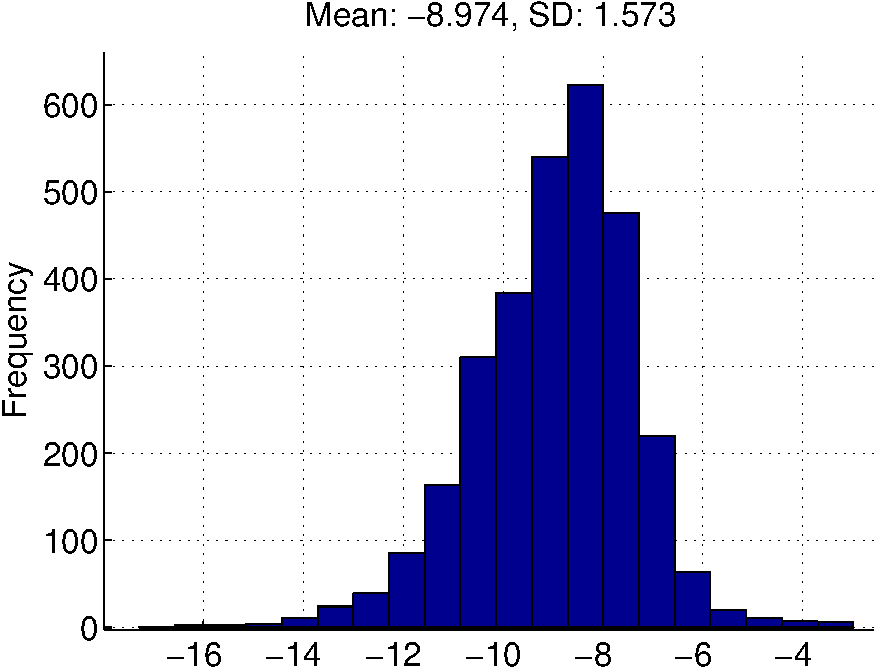
\includegraphics[width=6cm]{img/kl_ntr5000_iter5_sf1_st20_fm_joint-crop}
\par\end{centering}

\begin{centering}
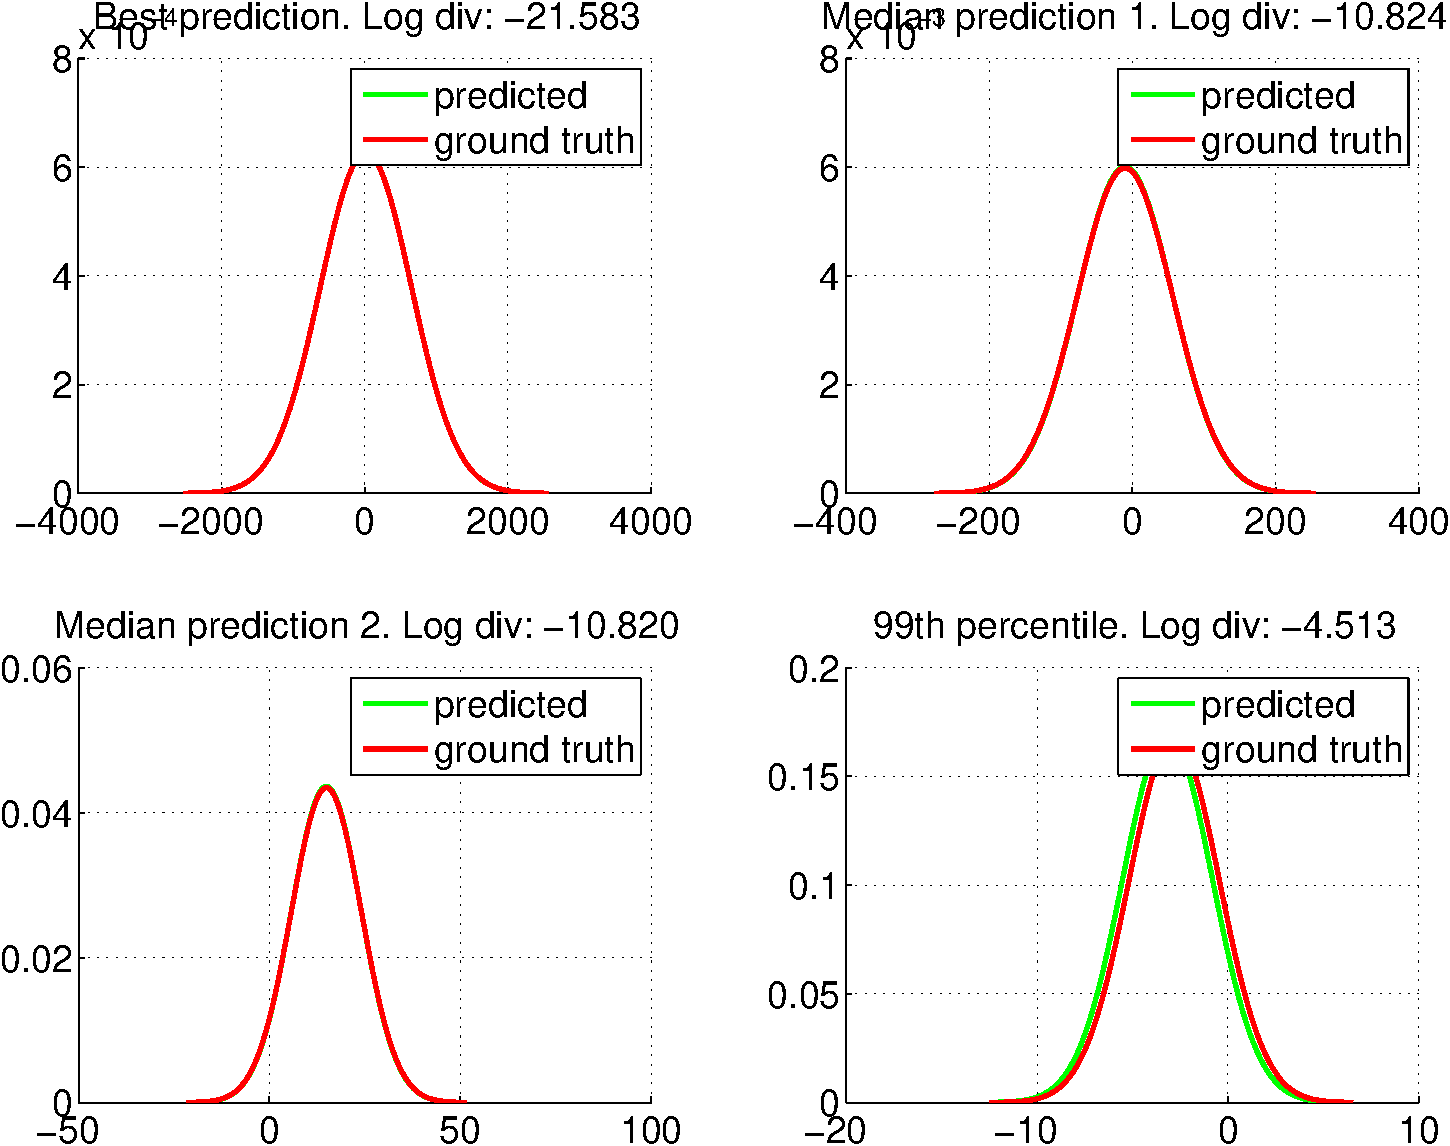
\includegraphics[width=6cm]{img/4plots_ntr5000_iter5_sf1_st20_fm_joint-crop.pdf}
\par\end{centering}

\protect\caption{KL-divergence on a logistic factor test set using kernel on joint
embeddings.\label{fig:Log-KL-divergence-on}}
\end{figure}

\paragraph{Compound Gamma}
\wjnote{Hopefully I will have enough time to do this.}

\subsection{Uncertainty Estimate}
In this experiment, we aim to verify that the predictive variance of the 
kernel-based message operator is a reliable quantity to be used as a criterion
for deciding whether or not to query the oracle.
We compute the predictive variance using the same operator as used in the logistic factor experiment on the training and test sets.
Plots of KL-divergence errors versus predictive variances are shown in \figref{fig:logistic_predvar}
, where the variance for predicting the mean of $m_{f \rightarrow X}$ is shown in \figref{fig:logistic_predvar_g}
and the variance for predicting $\log(\alpha)$ of $m_{f \rightarrow Z}$ is shown in \figref{fig:logistic_predvar_b}. 

\begin{figure}[t]
	\centering

	%DNormalLogVarBuilder means regressing to Gaussian mean and $\log$ variance.
	\subfloat[Predicting the mean of $m_{f \rightarrow X}$ (normal distribution)
	\label{fig:logistic_predvar_g}]{
	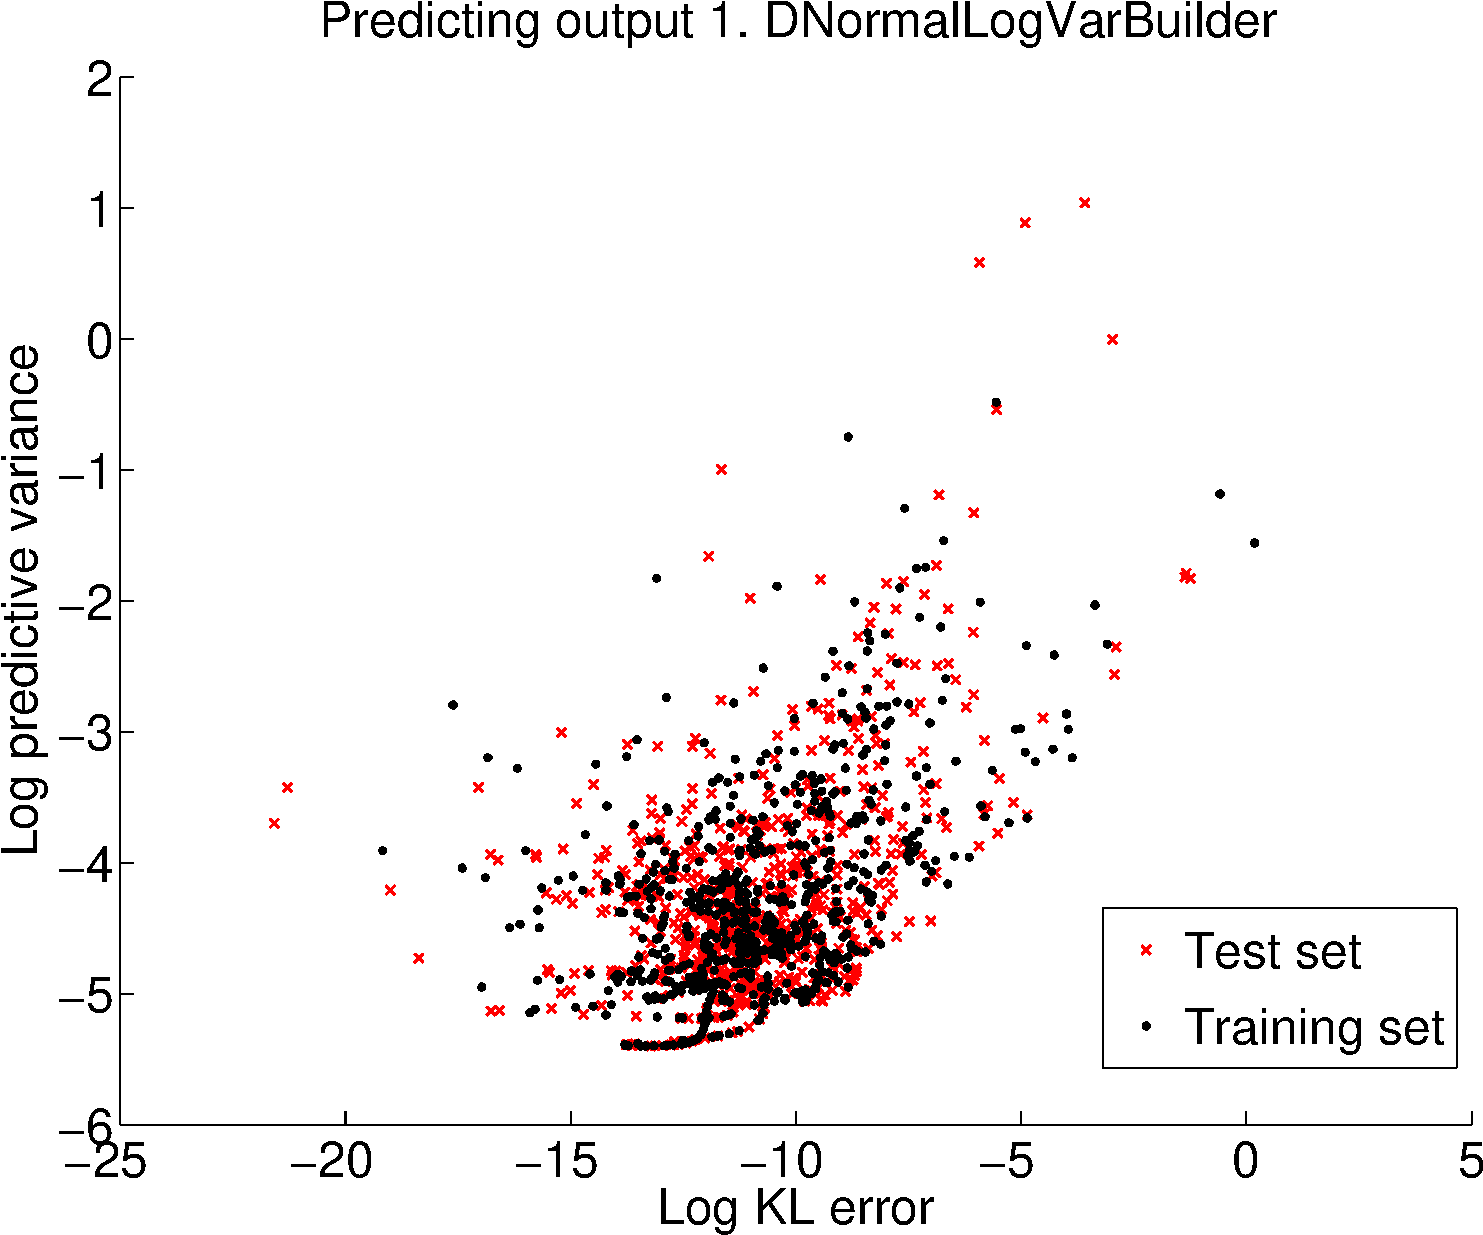
\includegraphics[width=0.7\columnwidth]{img/pred_var/fm_kgg_joint_-bw-out1-crop}
	}
	%\includegraphicse[width=7cm]{img/pred_var/fm_kgg_joint_-bw-out2-crop}
	
	\subfloat[Predicting $\log(\alpha)$ of $m_{f \rightarrow Z} = \text{Beta}(z; \alpha, \beta)$
	\label{fig:logistic_predvar_b}]{
	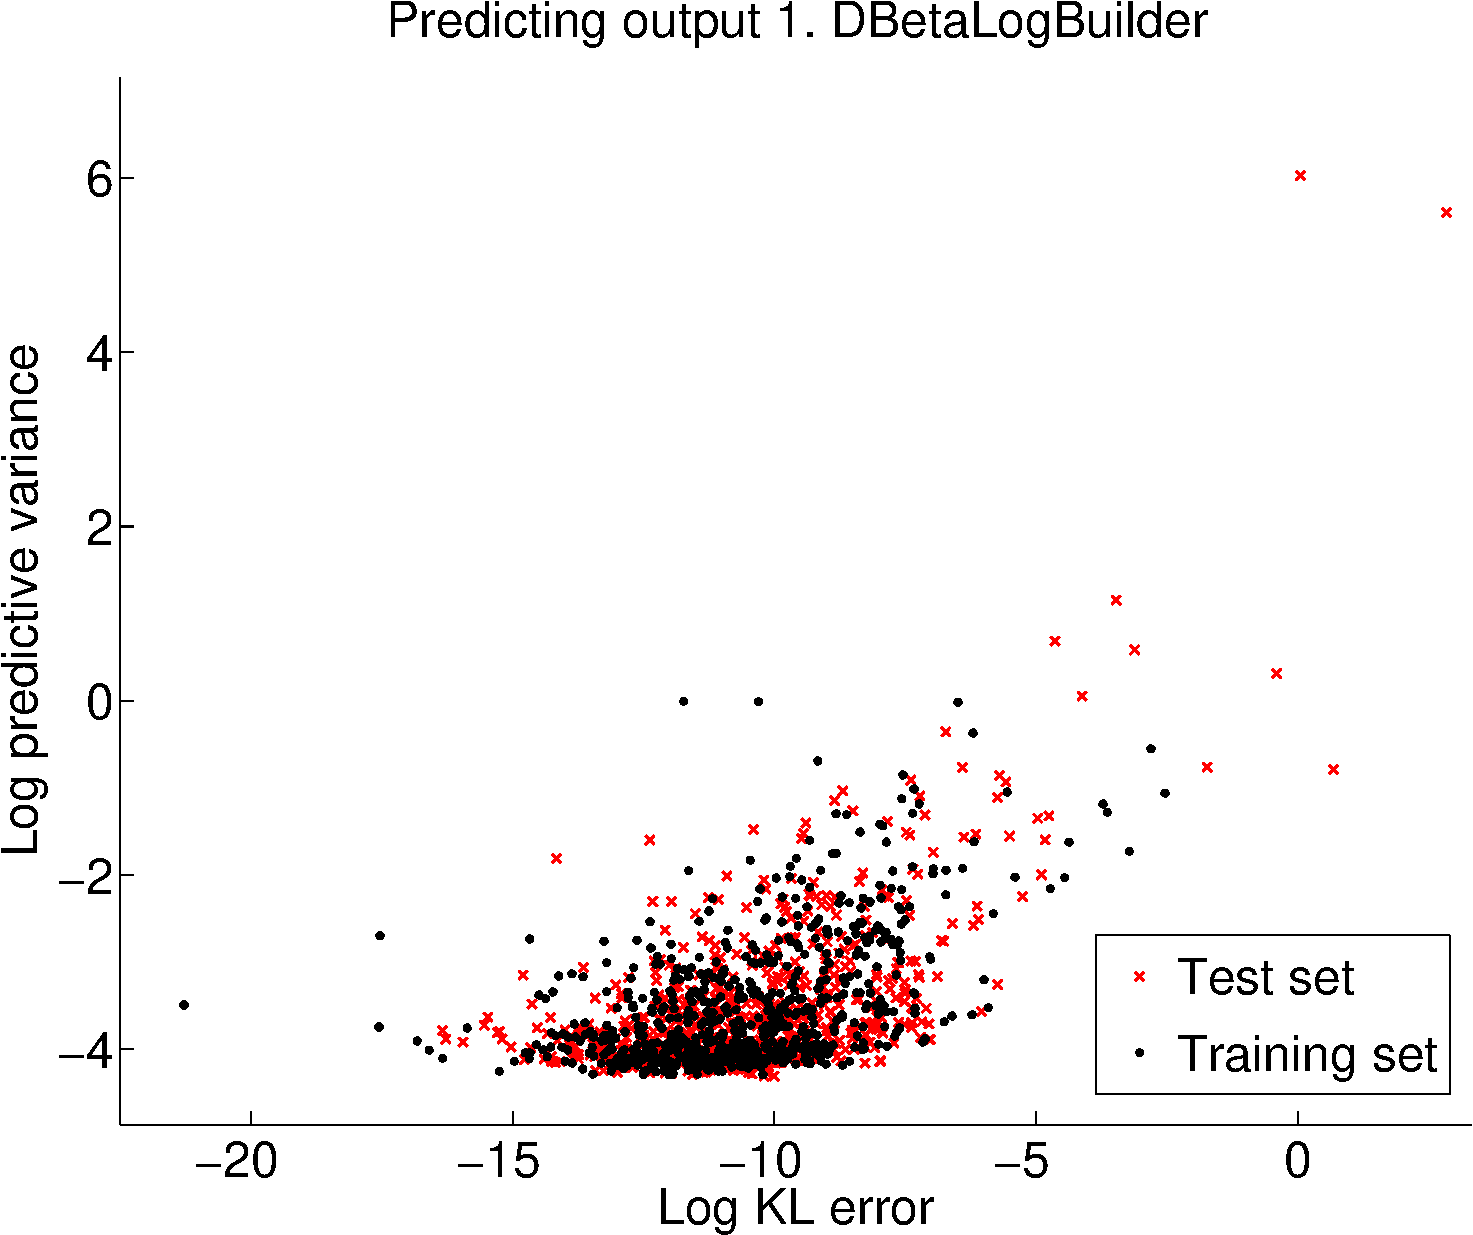
\includegraphics[width=0.7\columnwidth]{img/pred_var/fm_kgg_joint_-fw-out1-crop}
	}
	%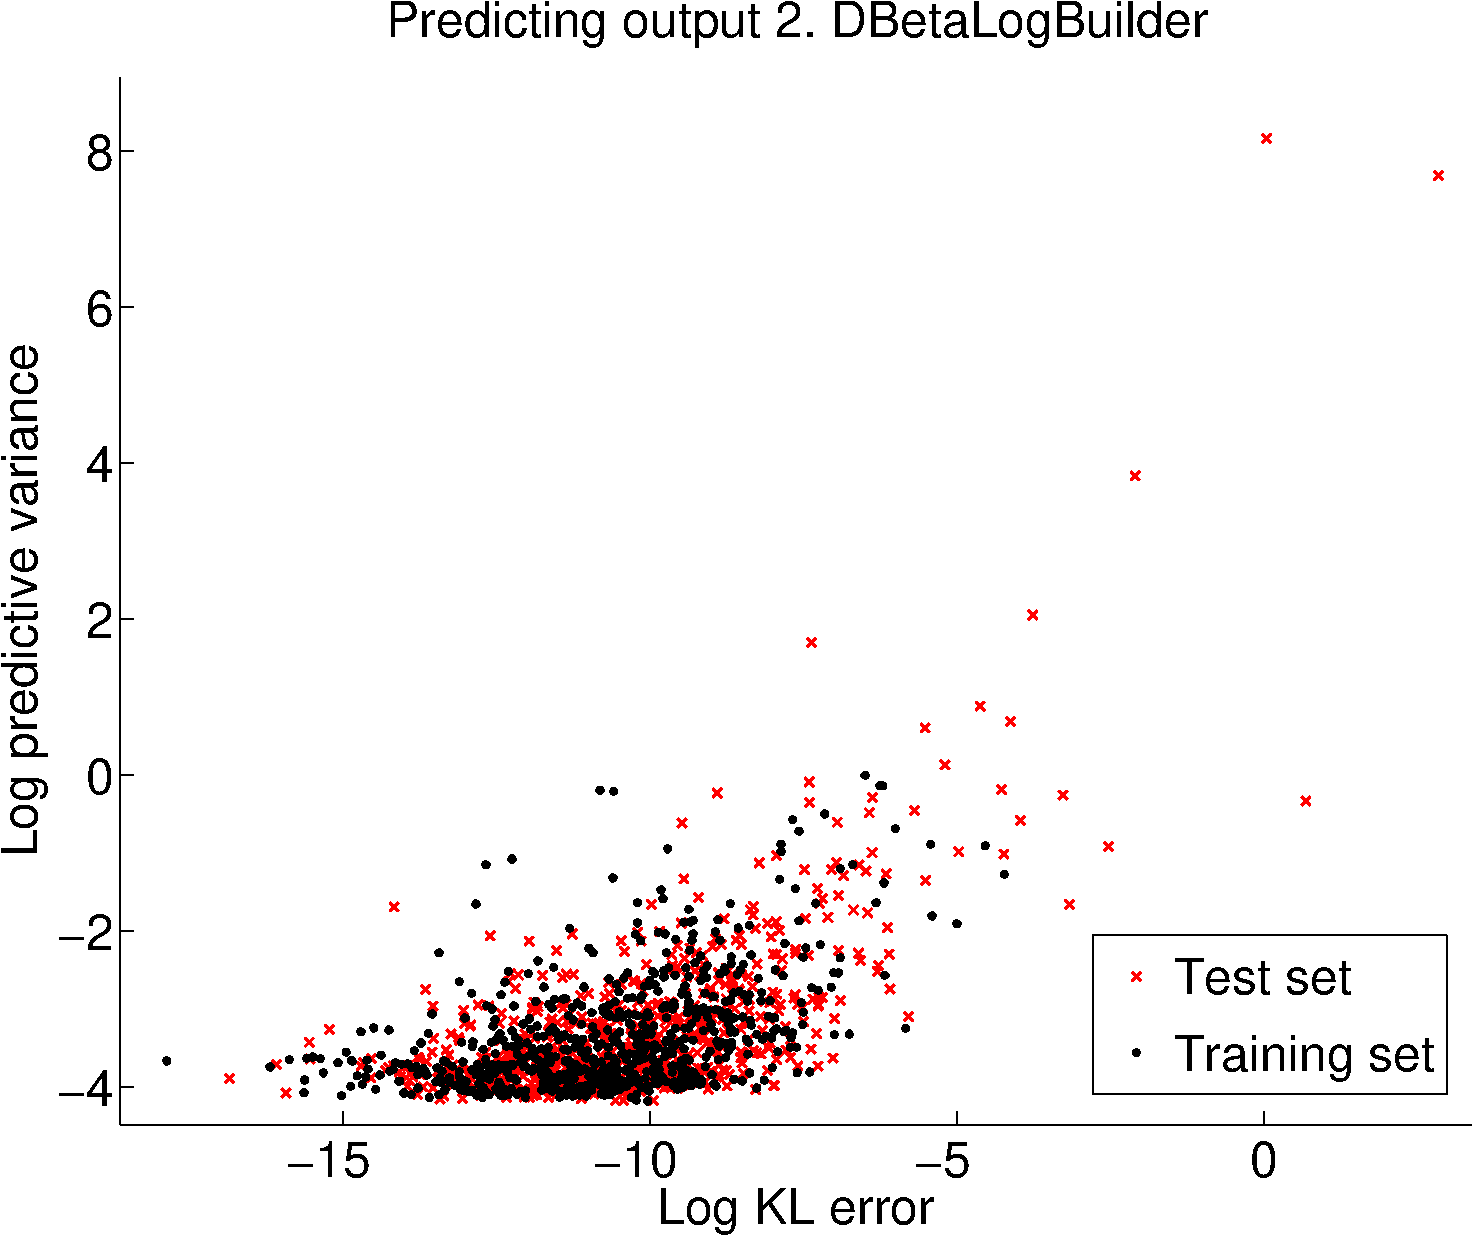
\includegraphics[width=7cm]{img/pred_var/fm_kgg_joint_-fw-out2-crop} 	
	\caption{KL-divergence errors versus predictive variances in the logistic factor problem.}
	\label{fig:logistic_predvar}
\end{figure}

\wjnote{Feel free to fill in more explanation.} 
The uncertainty estimates show a positive correlation with the KL-divergence errors. No points lie at the bottom right i.e., high confidence when it makes a big error.
No points lie at the top left i.e., not confident when it should not be.
The fact that the errors on the training set are roughly the same as the errors on the test set
indicates that the operator does not overfit.

\paragraph{Unexplored Region}
One of the most important tasks in JIT learning is to correctly estimate 
the predictive uncertainty in unexplored regions in the space of incoming messages. 
In this section, we show that the operator reports a high
uncertainty when encountered with incoming messages from a region far 
away from the messages in the training set. 
The first figure in \figref{fig:logistic_predvar_unexplored} shows the training set 
as used in the logistic factor experiment. Each point represents one incoming message
from $X$ i.e., $m_{X \rightarrow f}$. The incoming messages from $Z$ are not shown.
We consider two test sets represented as two curves in the first figure. 
The second figure in \figref{fig:logistic_predvar_unexplored} shows predict variance
of each point in the two test sets, where we fix $m_{Z \rightarrow f} := \text{Beta}(z; 1, 2)$.

\wjnote{Finish this explanation. Two key observations. 1. As a test point lies further away
from the training set, the predictive variance grows exponentially.
2. In both test sets, the operator is most certain around zeros mean. 
However, the first test set passes through a lower density region, the operator 
reports a higher uncertainty compared to the second test set. }

Uncertainty estimates from two commonly used random forests on the 
same problem are shown in \figref{fig:tree_uncertainty_unexplored} where
\figref{fig:breiman_uncertainty} shows uncertainty estimates of Breiman's 
random forests \citep{Breiman2001} and \figref{fig:ert_uncertainty} shows 
uncertainty estimates of extremely randomized trees \citep{Geurts2006}.
We set the number of trees to 100 in both cases and other parameters to 
the default settings as set in Scikit-learn package \citep{Pedregosa2011}. 

\wjnote{Need to add how they compute the uncertainty estimates. ?}
\wjnote{Add comments on uncertainty estimates of the trees.}

\begin{figure}
\centering
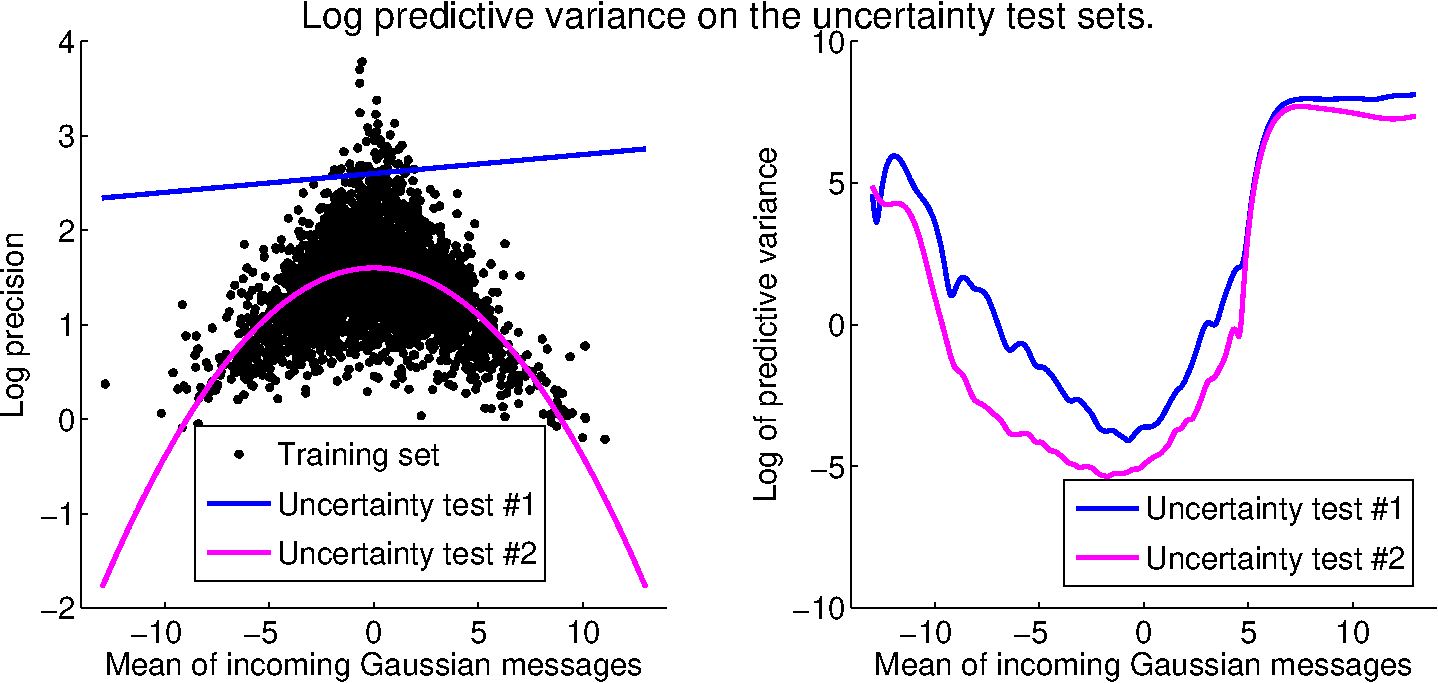
\includegraphics[width=\columnwidth]{img/uncertainty/logistic_uncertainty-crop}
\caption{Collected training messages for the logistic factor and uncertainty 
estimates of the proposed method on the two uncertainty test sets.}
\label{fig:logistic_predvar_unexplored}
\end{figure}


\begin{figure}[t]
	\centering

	\subfloat[Breiman's random forests\label{fig:breiman_uncertainty}]{
	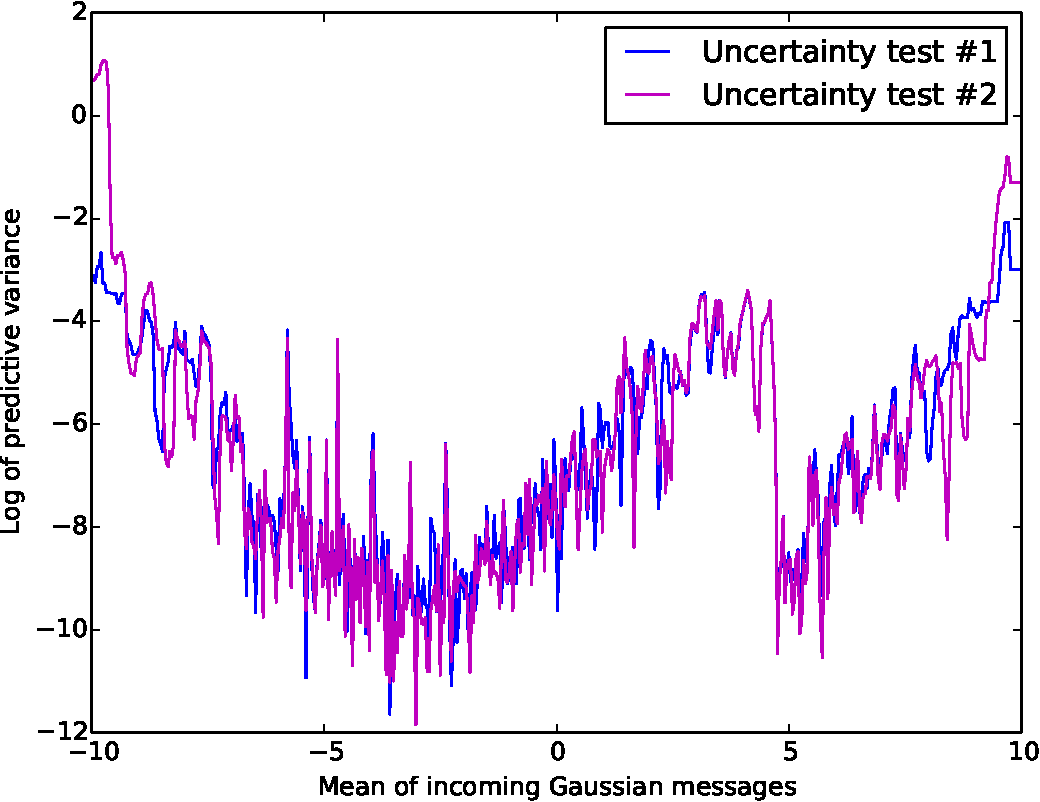
\includegraphics[width=0.49\columnwidth]{img/uncertainty/rf-n_trees-100-crop}
	}
	%
	\subfloat[Extremely randomized trees\label{fig:ert_uncertainty}]{
	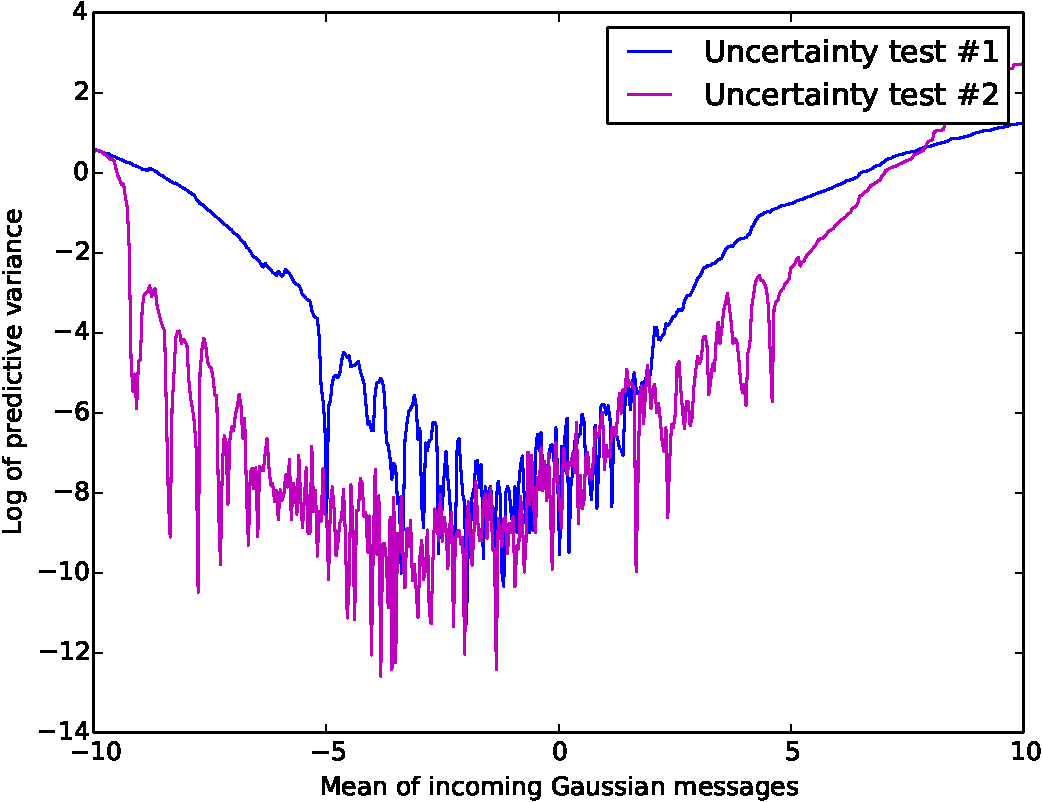
\includegraphics[width=0.49\columnwidth]{img/uncertainty/ert-n_trees-100-crop}
	}
	\caption{Uncertainty estimates of random forests on two uncertainty test sets 
	shown in \figref{fig:logistic_predvar_unexplored}. }
	\label{fig:tree_uncertainty_unexplored}
\end{figure}

%\begin{figure}
%\centering
%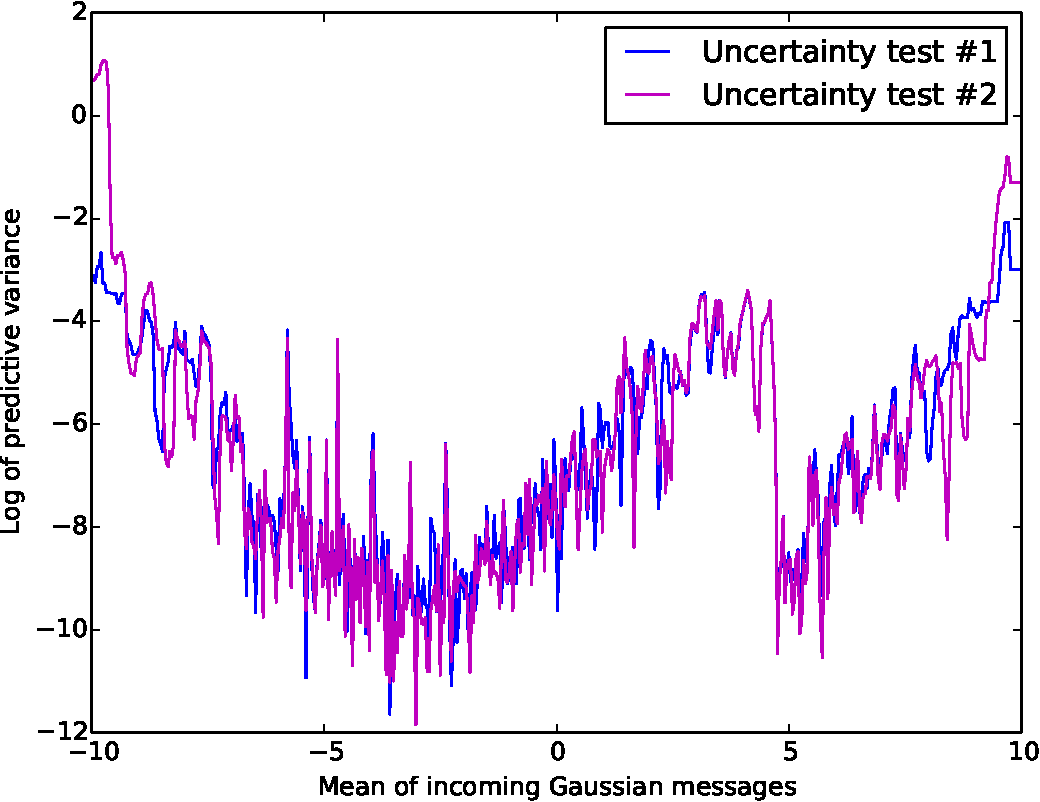
\includegraphics[width=0.49\columnwidth]{img/uncertainty/rf-n_trees-100-crop}
%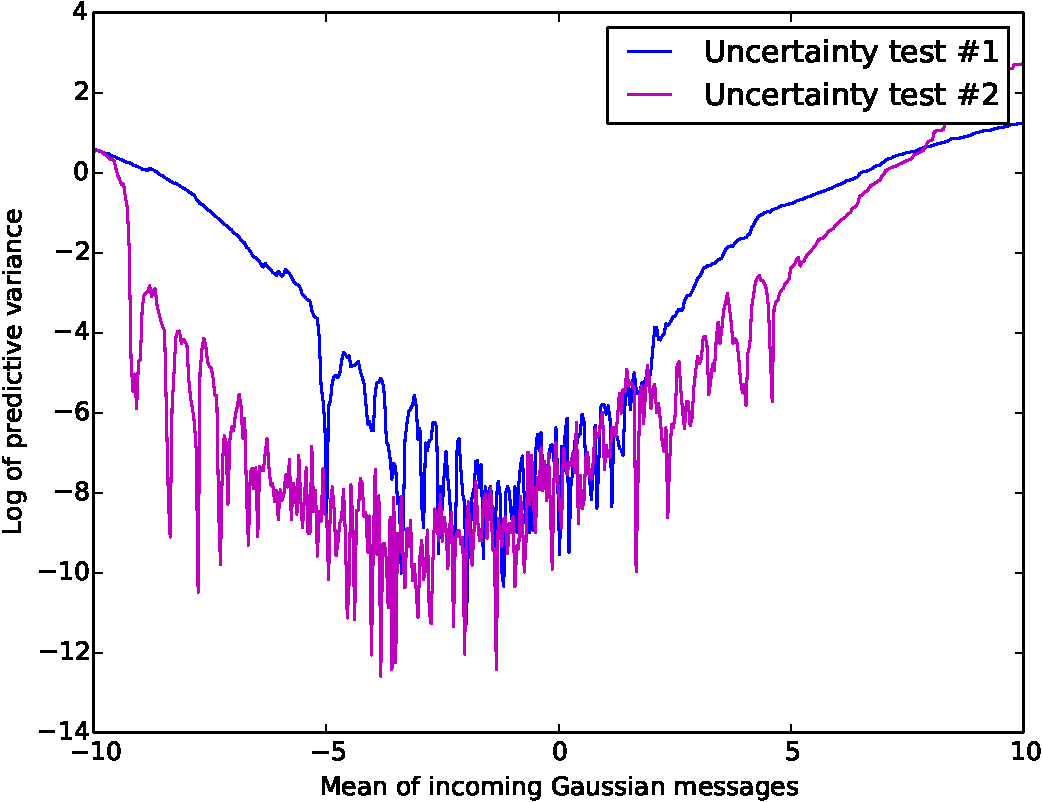
\includegraphics[width=0.49\columnwidth]{img/uncertainty/ert-n_trees-100-crop}
%\caption{Log KL-divergence on a logistic factor test set using kernel on joint embeddings.}
%\label{fig:tree_uncertainty_unexplored}
%\end{figure}


\hrulefill{}

\hl{Experiments to have}
\begin{itemize}
\item For predictive variance on unseen region, we may need two plots where
in one case the training samples are concentrated in one part of the
space, and in the second case the training samples are concentrated
in another part. This is to ensure that the uncertainty estimate does
not depend on the absolute location.
\item Use the operator for logistic in a binary logistic regression problem
with a real dataset. Compare the inferred posterior of the coefficient
vector to the posterior obtained by the handcrafted message operator,
possibly with a histogram of log KL (of posteriors).
\item Experiments on compound gamma factor whose handcrafted operator is
slow. We can show that using a regression-based operator can be faster
and possibly more accurate. A compound gamma can be used as a prior
on a Gaussian precision in some model. Would be nice to have a real
dataset (say a binary classification dataset from UCI repository).
\item A table comparing performance of different kernels. Put in the main 
text if there is space.

\begin{itemize}
\item Andrew Gelman \citep{Gelman2006}, Tom Minka: ``Gamma prior on precision
is not good''. Cite them.
\end{itemize}
%\item Do we need kNN as a baseline regression function? \aenote{AE: Maybe enough to point to JIT paper and say KNN performs badly there?}
\item Choose the number of particles in the oracle importance sampler so
that it takes roughly the same time as our operator. Compute the predictive
quality of the two. 
\item As in Fig 3.c of Ali's paper, show that the inference error of sampling
+ JIT is better than sampling alone. This asserts that JIT interpolates
in the message space in a useful way. \aenote{AE: This would be nice but is probably not critical. Could be one of the last experiments you run?}
\end{itemize}

\hrule 

%\subsection*{Acknowledgement}
%Thank Balaji for testing uncertainty estimates of random forests.
%Gatsby Charitable Foundation for funding.

\section{Conclusions and Future Work\label{sec:Conclusions-and-Future} }

We propose to learn to send EP messages with kernel ridge regression
by casting the KL minimization problem as a supervised learning problem.
With random features, incoming messages to a learned operator are
converted to a finite-dimensional vector. Computing an outgoing message
amounts to computing the moment parameters by multiplying the vector
with a matrix given by the solution of the primal ridge regression.

\bibliographystyle{abbrvnat}
\bibliography{ref}


\newpage

\onecolumn

\appendix

\begin{center}
\textbf{\textcolor{black}{\LARGE{}Supplementary Materials}}
\par\end{center}{\LARGE \par}

\todo[inline]{The following incoherent content needs to be rewritten. I just copied it from my notes. Some part will be moved to the main text.  }




\section{Kernel Ridge Regression}


\subsection{Kernel Ridge Regression in Primal Form}

In our work, we can apply random features to the kernel in the conditional
mean embedding operator. With $\hat{\phi}$, an estimate of an operator
in primal solution is
\begin{align*}
\hat{C}_{x'|w} & =X'W^{\top}\left(WW^{\top}+\lambda I\right)^{-1}\\
 & \approx\underbrace{X'}_{d_{x}\times N}\underbrace{\hat{\Phi}^{\top}}_{N\times D}\underbrace{\left(\hat{\Phi}\hat{\Phi}^{\top}+\lambda I\right)^{-1}}_{D\times D}
\end{align*}
where $\hat{\Phi}=\left(\hat{\phi}(w_{1})|\cdots|\hat{\phi}(w_{N})\right)\in\mathbb{R}^{D\times N}$
and $W=X\otimes Y$ . So an estimated operator can be represented
with a $d_{x}\times D$ matrix where $d_{x}$ is the dimension of
the target sufficient statistic. Applying the operator to a test message
$m_{w\rightarrow f}^{*}$ with random features given by $\phi^{*}\in\mathbb{R}^{D}$
requires just a matrix vector multiplication whose complexity does
not depend on $N$ (unlike in the dual form).


\subsection{Leave-One-Out Cross Validation with Random Features\label{sub:LOOCV-for-Operator}}

The solution of the kernel ridge regression is given by
\[
\hat{C}_{Y|X}=YX^{\top}\left(XX^{\top}+\lambda I\right)^{-1}
\]
where $Y\in\mathbb{R}^{d_{y}\times n}$ and $d_{y}$ is the number
of sufficient statistic outputs i.e., two for a one-dimensional Gaussian.
With random features, we have $K_{ij}\approx\hat{\phi}_{i}^{\top}\hat{\phi}_{j}:=\hat{\phi}(x_{i})^{\top}\hat{\phi}(x_{j})$
where $\hat{\phi}_{i}\in\mathbb{R}^{d}$ and $d$ is the number of
random features. In our work, $x_{i}$ will be an instance in the
tensor product space of the form $x_{i}=m_{x_{1}\rightarrow f}\otimes m_{x_{2}\rightarrow f}\otimes\cdots$.
So the estimator can be rewritten as
\[
\hat{C}_{Y|X}\approx\underbrace{Y}_{d_{y}\times n}\underbrace{\hat{\Phi}^{\top}}_{n\times d}\underbrace{\left(\hat{\Phi}\hat{\Phi}^{\top}+\lambda I\right)^{-1}}_{d\times d}
\]
where $\hat{\Phi}:=\left(\hat{\phi}_{1}|\cdots|\hat{\phi}_{n}\right)\in\mathbb{R}^{d\times n}$.
The LOOCV error can be written as
\[
E_{LOOCV}:=\frac{1}{n}\sum_{j=1}^{n}\|\hat{C}_{Y|X}^{(j)}\hat{\phi}_{j}-y_{j}\|_{d_{y}}^{2}
\]
where $\hat{C}_{Y|X}^{(j)}$ is the estimator obtained with $j^{th}$
instance removed and $y_{j}\in\mathbb{R}^{d_{y}}$. Following the
same idea as in the ordinary ridge regression, we express $\hat{C}_{Y|X}^{(j)}$
in terms of $\hat{C}_{Y|X}$.
\begin{align*}
\hat{C}_{Y|X}^{(j)} & =\left(Y\hat{\Phi}-y_{j}\phi_{j}^{\top}\right)\left(\hat{\Phi}\hat{\Phi}^{\top}+\lambda I-\hat{\phi}_{j}\hat{\phi}_{j}^{\top}\right)^{-1}\\
 & =\left(Y\hat{\Phi}-y_{j}\phi_{j}^{\top}\right)\left(A^{-1}+\frac{A^{-1}\phi_{j}\phi_{j}^{\top}A^{-1}}{1-\phi_{j}^{\top}A^{-1}\phi_{j}}\right)\\
 & =\hat{C}_{Y|X}+h_{jj}^{-1}YL\phi_{j}\phi_{j}^{\top}A^{-1}-h_{jj}^{-1}y_{j}\phi_{j}^{\top}A^{-1}
\end{align*}
where $h_{ii}:=\left(H\right)_{ii}=1-\phi_{i}^{\top}A^{-1}\phi_{i}$,
$A:=\hat{\Phi}\hat{\Phi}^{\top}+\lambda I$ and $L:=\hat{\Phi}^{\top}A^{-1}$.
Note that with these definitions, we have $\hat{C}_{Y|X}=YL$. By
plugging $\hat{C}_{Y|X}^{(j)}$ back to $E_{LOOCV}$, we have
\begin{align*}
E_{LOOCV} & =\frac{1}{n}\sum_{j=1}^{n}\bigg\|\hat{C}_{Y|X}\hat{\phi}_{j}+h_{jj}^{-1}YL\hat{\phi}_{j}\underbrace{\hat{\phi}_{j}^{\top}A^{-1}\hat{\phi}_{j}}_{1-h_{jj}}-h_{jj}^{-1}y_{j}\underbrace{\hat{\phi}_{j}A^{-1}\hat{\phi}_{j}}_{1-h_{jj}}-y_{j}\bigg\|^{2}\\
 & =\frac{1}{n}\sum_{j=1}^{n}\bigg\|\hat{C}_{Y|X}\hat{\phi}_{j}+\left(h_{jj}^{-1}-1\right)YL\hat{\phi}_{j}-\left(h_{jj}^{-1}-1\right)y_{j}-y_{j}\bigg\|_{d_{y}}^{2}\\
 & =\frac{1}{n}\bigg\|\underbrace{\hat{C}_{Y|X}}_{YL}\hat{\Phi}+YL\hat{\Phi}\left(\tilde{H}^{-1}-I\right)-Y\tilde{H}^{-1}\bigg\|_{F}^{2}\\
 & =\frac{1}{n}\bigg\| YL\hat{\Phi}\tilde{H}^{-1}-Y\tilde{H}^{-1}\bigg\|_{Y}^{2}=\frac{1}{n}\bigg\| Y\left(L\hat{\Phi}-I\right)\tilde{H}^{-1}\bigg\|_{F}^{2}\\
 & =\frac{1}{n}\bigg\| YH\tilde{H}^{-1}\bigg\|_{F}^{2}
\end{align*}
where $H:=I-L\hat{\Phi}=I-\hat{\Phi}^{\top}\left(\hat{\Phi}\hat{\Phi}^{\top}+\lambda I\right)^{-1}\hat{\Phi}\in\mathbb{R}^{n\times n}$,
$\tilde{H}$ is a diagonal matrix with the same diagonal as $H$ and
$\|A\|_{F}^{2}:=\trace\left(A^{\top}A\right)$ is the squared Frobenius
norm.


\paragraph{Computing $E_{LOOCV}$}

In computing $E_{LOOCV}$, one should not form $H\in\mathbb{R}^{n\times n}$
explicitly because $n$ is assumed to be huge. 
\begin{align*}
\bigg\| YH\tilde{H}^{-1}\bigg\|_{F}^{2} & =\trace\left(YH\tilde{H}^{-2}H^{\top}Y^{\top}\right)\\
 & =\trace\left(Y\tilde{H}^{-2}Y^{\top}-Y\tilde{H}^{-2}\hat{\Phi}^{\top}A^{-1}\hat{\Phi}Y^{\top}-Y\hat{\Phi}^{\top}A^{-1}\hat{\Phi}\tilde{H}^{-2}Y^{\top}+Y\hat{\Phi}^{\top}A^{-1}\hat{\Phi}\tilde{H}^{-2}\hat{\Phi}^{\top}A^{-1}\hat{\Phi}Y^{\top}\right)
\end{align*}
Let $E:=Y\hat{\Phi}^{\top}A^{-1}\hat{\Phi}\in\mathbb{R}^{d_{y}\times n},B=Y\tilde{H}^{-1}\in\mathbb{R}^{d_{y}\times n}$
then the last line becomes
\begin{align*}
 & \trace\left(BB^{\top}-B\tilde{H}^{-1}E^{\top}-E\tilde{H}^{-1}B^{\top}+E\tilde{H}^{-2}E^{\top}\right)\\
= & \trace\left(BB^{\top}\right)-2\trace\left(E\tilde{H}^{-1}B^{\top}\right)+\trace\left(E\tilde{H}^{-2}E^{\top}\right).
\end{align*}
 Each term in the trace is of size $d_{y}\times d_{y}$. This does
not involve forming an $n\times n$ matrix. $\tilde{H}$ is the diagonal
of $H$. So, $\tilde{H}=\diag\left(I-\hat{\Phi}^{\top}A^{-1}\hat{\Phi}\right)$.
The cost of $O(d^{3})$ seems to be inevitable where $d$ is expected
to be in the order of thousands. The number is large enough that $d^{3}$
is expensive. In computing $E_{LOOCV}$ for selecting the best parameter
combination, we may reduce $d$. The number of features $d$ is set
back to the desired value during testing. 


\paragraph{Operator representation}

Once the best parameter combination is choosen, we increase $d$ to
the desired value and precompute $\hat{C}_{Y|X}\approx\underbrace{Y}_{d_{y}\times n}\underbrace{\hat{\Phi}^{\top}}_{n\times d}\underbrace{\left(\hat{\Phi}\hat{\Phi}^{\top}+\lambda I\right)^{-1}}_{d\times d}$
for test time. One obvious improvement is to avoid forming $\hat{\Phi}$
explicitly since the memory cost will be $O(dn)$ which can already
be huge. $Y\hat{\Phi}$ can be computed incrementally without the
need to form $\hat{\Phi}$. Memory cost for computing $\hat{\Phi}\hat{\Phi}^{\top}$
can be made lower than $O(dn)$ by computing incrementally even though
the computational complexity remains $O(dn^{2})$ which is still huge.
The total cost for computing the operator is $O(d^{2}n+d^{3})$. Linear
dependency on $n$ is unavoidable. 


\section{Kernels and Random Features}

This section reviews relevant kernels and their random feature representations.


\subsection{Random Features}

This section contains a summary of \citesup{Rahimi2007}'s random
Fourier features for a translation invariant kernel. 

A kernel $k(x,y)=\left\langle \phi(x),\phi(y)\right\rangle $ in general
may correspond to an inner product in an infinite-dimensional space
whose feature map $\phi$ cannot be explicitly computed. In \citesup{Rahimi2007},
methods of computing an approximate feature maps $\hat{\phi}$ were
proposed. The approximate feature maps are such that $k(x,y)\approx\hat{\phi}(x)^{\top}\hat{\phi}(y)$
(with equality in expectation) where $\hat{\phi}\in\mathbb{R}^{D}$
and $D$ is the number of random features. High $D$ yields a better
approximation with higher computational cost. Assume $k(x,y)=k(x-y)$
and $x,y\in\mathbb{R}^{d}$. Random Fourier features $\hat{\phi}(x)\in\mathbb{R}^{D}$
such that $k(x,y)\approx\hat{\phi}(x)^{\top}\hat{\phi}(y)$ are generated
as follows.
\begin{enumerate}
\item Compute the Fourier transform $\hat{k}$ of the kernel $k$: $\hat{k}(\omega)=\frac{1}{2\pi}\int e^{-j\omega^{\top}\delta}k(\delta)\, d\delta$.
For a Gaussian kernel with unit width, $\hat{k}(\omega)=\left(2\pi\right)^{-d/2}e^{-\|\omega\|^{2}/2}$.
\item Draw $D$ i.i.d. samples $\omega_{1},\ldots,\omega_{D}\in\mathbb{R}^{d}$
from $\hat{k}$. 
\item Draw $D$ i.i.d samples $b_{1},\ldots,b_{D}\in\mathbb{R}$ from $U[0,2\pi]$
(uniform distribution).
\item $\hat{\phi}(x)=\sqrt{\frac{2}{D}}\left(\cos\left(\omega_{1}^{\top}x+b_{1}\right),\ldots,\cos\left(\omega_{D}^{\top}x+b_{D}\right)\right)^{\top}\in\mathbb{R}^{D}$
\end{enumerate}

\paragraph{Why it works ?}
\begin{thm}
Bochner's theorem. A continuous kernel $k(x,y)=k(x-y)$ on $\mathbb{R}^{m}$
is positive definite iff $k(\delta)$ is the Fourier transform of
a non-negative measure.
\end{thm}
Furthermore, if a translation invariant kernel $k(\delta)$ is properly
scaled, Bochner's theorem guarantees that its Fourier transform $p(\omega)$
is a proper probability distribution. From this fact, we have 
\[
k(x-y)=\int\hat{k}(\omega)e^{j\omega^{\top}\left(x-y\right)}\, d\omega=\mathbb{E}_{\omega}\left[\eta_{\omega}(x)\eta_{\omega}(y)^{*}\right]
\]
where $\eta_{\omega}(x)=e^{j\omega^{\top}x}$ and $\cdot^{*}$ denotes
the complex conjugate. Since both $p$ and $k$ are real, the complex
exponential contains only the cosine terms. Drawing $d$ samples is
for lowering the variance of the approximation.
\begin{thm}
\label{thm:Separation-of-variables.}Separation of variables. Let
$\hat{f}$ be the Fourier transform of $f$. If $f(x_{1},\ldots,x_{n})=f_{1}(x_{1})\cdots f_{n}(x_{n})$,
then $\hat{f}(\omega_{1},\ldots,\omega_{n})=\prod_{i=1}^{n}\hat{f}_{i}(\omega_{i})$. 
\end{thm}
Theorem \ref{thm:Separation-of-variables.} suggests that the random
Fourier features can be extended to product kernel by drawing $\omega$
independently for each kernel. 


\subsection{MV (Mean-Variance) Kernel}

Assume there are $c$ incoming messages $\left(p^{(i)}\right)_{i=1}^{c}$
. Assume that
\begin{align*}
\mathbb{E}_{p^{(l)}}\left[x\right] & =m_{l}\\
\mathbb{V}_{p^{(l)}}\left[x\right] & =v_{l}\\
\mathbb{E}_{q^{(l)}}\left[y\right] & =\mu_{l}\\
\mathbb{V}_{q^{(l)}}\left[y\right] & =\sigma_{l}^{2}.
\end{align*}
We use $p^{(l)}(x)$ and $m_{x_{i}\rightarrow f}(x)$ interchageably.
Incoming messages are not necessarily Gaussian. They do have to be
in the exponential family. MV (mean-variance) kernel is a a product
kernel on means and variances. 
\begin{align*}
\kappa\left(\left(p^{(i)}\right)_{i=1}^{c},\left(q^{(i)}\right)_{i=1}^{c}\right) & =\prod_{i=1}^{c}\kappa^{(i)}\left(p^{(i)},q^{(i)}\right)\\
 & =\prod_{i=1}^{c}k\left(\left(m_{i}-\mu_{i}\right)/w_{i}^{m}\right)\prod_{i=1}^{c}k\left(\left(v_{i}-\sigma_{i}^{2}\right)/w_{i}^{v}\right)
\end{align*}
where $k$ is a Gassian kernel with unit width. The kernel $\kappa$
has $P:=\left(w_{1}^{m},\ldots,w_{c}^{m},w_{1}^{v},\ldots,w_{c}^{v}\right)$
as its parameters. With this kernel, we treat messages as finite dimensional
vector. All incoming messages $(q^{(i)})_{i=1}^{c}$ are essentially
represented as $\left(\mu_{1},\ldots,\mu_{c},\sigma_{1}^{2},\ldots,\sigma_{c}^{2}\right)^{\top}$.
This treatment reduces the problem of having distributions as inputs
to the familiar problem of having input points from a Euclidean space.
The random features of \cite{Rahimi2007} can be applied straightforwardly. 


\subsection{Expected Product Kernel\label{sub:Expected-Product-Kernel}}

Let $\mu_{r^{(l)}}:=\mathbb{E}_{r^{(l)}(a)}k(\cdot,a)$ be the mean
embedding \citepsup{Smola2007} of the distribution $r^{(l)}$ into
RKHS $\mathcal{H}^{(l)}$ induced by the kernel $k$. Assume $k=k_{\text{gauss}}$
(Gaussian kernel) and assume there are $c$ incoming messages $\mathsf{x}:=(r^{(i)}(a^{(i)}))_{i=1}^{c}$
and $\mathsf{y}:=(s^{(i)}(b^{(i)}))_{i=1}^{c}$. An expected product
kernel $\kappa_{\text{pro}}$ is defined as 
\begin{align*}
\kappa_{\text{pro}}\left(\mathsf{x},\mathsf{y}\right) & :=\left\langle \bigotimes_{l=1}^{c}\mu_{r^{(l)}},\bigotimes_{l=1}^{c}\mu_{s^{(l)}}\right\rangle _{\otimes_{l}\mathcal{H}^{(l)}}=\prod_{l=1}^{c}\mathbb{E}_{r^{(l)}(a)}\mathbb{E}_{s^{(l)}(b)}k_{\text{gauss}}^{(l)}\left(a,b\right)\approx\hat{\phi}(\mathsf{x})^{\top}\hat{\phi}(\mathsf{y})
\end{align*}
where $\hat{\phi}(\mathsf{x})^{\top}\hat{\phi}(\mathsf{y})=\prod_{l=1}^{c}\hat{\phi}^{(l)}(r^{(l)})^{\top}\hat{\phi}^{(l)}(s^{(l)})$.
The feature map $\hat{\phi}^{(l)}(r^{(l)})$ can be estimated by applying
the random Fourier features to $k_{\text{gauss }}^{(l)}$and taking
the expectations $\mathbb{E}_{r^{(l)}(a)}\mathbb{E}_{s^{(l)}(b)}$.
The final feature map is $\hat{\phi}(\mathsf{x})=\hat{\phi}^{(1)}(r^{(1)})\circledast\hat{\phi}^{(2)}(r^{(2)})\circledast\cdots\circledast\hat{\phi}^{(c)}(r^{(c)})\in\mathbb{R}^{d^{c}}$where
$\circledast$ denotes a Kronecker product and we assume that $\hat{\phi}^{(l)}\in\mathbb{R}^{d}$
for $l\in\{1,\ldots,c\}$. 

We first give some results which will be used to derive the Fourier
features for inner product of mean embeddings.
\begin{lem}
If $b\sim\mathcal{N}(b;0,\sigma^{2})$, then $\mathbb{E}[\cos(b)]=\exp\left(-\frac{1}{2}\sigma^{2}\right)$.\label{lemma:e_cos}\end{lem}
\begin{proof}
We can see this by considering the characteristic function of $x\sim\mathcal{N}(x;\mu,\sigma^{2})$
which is given by $c_{x}(t)$.
\[
c_{x}(t)=\mathbb{E}_{x}\left[\exp\left(itb\right)\right]=\exp\left(itm-\frac{1}{2}\sigma^{2}t^{2}\right)
\]
For $m=0,t=1$, we have 
\[
c_{b}(1)=\mathbb{E}_{b}\left[\exp(ib)\right]=\exp\left(-\frac{1}{2}\sigma^{2}\right)=\mathbb{E}_{b}\left[\cos(b)\right]
\]
where we have $\cos()$ because the imaginary part is set to 0 i.e.,
$i\sin(tb)$ vanishes.
\end{proof}
Given two messages $p(x)=\mathcal{N}(x;m_{p},V_{p})$ and $q(y)=\mathcal{N}(y;m_{q},V_{q})$
($d$-dimensional Gaussian), the expected product kernel is defined
as 
\[
\kappa(p,q)=\left\langle \mu_{p},\mu_{q}\right\rangle _{\mathcal{H}}=\mathbb{E}_{p}\mathbb{E}_{q}k(x-y)
\]
where $\mu_{p}:=\mathbb{E}_{p}k(x,\cdot)$ is the mean embedding of
$p$ and we assume that the kernel $k$ associated with $\mathcal{H}$
is translation invariant i.e.g, $k(x,y)=k(x-y)$. The goal here is
to derive random Fourier features for the expected product kernel.
That is, we aim to find $\hat{\phi}$ such that $\kappa(p,q)\approx\hat{\phi}(p)^{\top}\hat{\phi}(q)$
and $\hat{\phi}\in\mathbb{R}^{D}$. 

From \cite{Rahimi2007} which provides random features for $k(x-y)$,
we immediately have
\begin{align*}
\mathbb{E}_{p}\mathbb{E}_{q}k(x-y) & \approx\mathbb{E}_{p}\mathbb{E}_{q}\frac{2}{D}\sum_{i=1}^{D}\cos\left(w_{i}^{\top}x+b_{i}\right)\cos\left(w_{i}^{\top}y+b_{i}\right)\\
 & =\frac{2}{D}\sum_{i=1}^{D}\mathbb{E}_{p(x)}\cos\left(w_{i}^{\top}x+b_{i}\right)\mathbb{E}_{q(y)}\cos\left(w_{i}^{\top}y+b_{i}\right)
\end{align*}
where $\{w_{i}\}_{i=1}^{D}\sim\hat{k}(w)$ (Fourier transform of $k$)
and $\{b_{i}\}_{i=1}^{D}\sim U\left[0,2\pi\right]$. 

Consider $\mathbb{E}_{p(y)}\cos\left(w_{i}^{\top}x+b_{i}\right)$.
Define $z_{i}=w_{i}^{\top}x+b_{i}$. So $z_{i}\sim\mathcal{N}(z_{i};w_{i}^{\top}m_{p}+b_{i},w_{i}^{\top}V_{p}w_{i})$.
Let $d_{i}\sim\mathcal{N}(0,w_{i}^{\top}V_{p}w_{i})$. Then, $p(d_{i}+w_{i}^{\top}m_{p}+b_{i})=\mathcal{N}(w_{i}^{\top}m_{p}+b_{i},w_{i}^{\top}V_{p}w_{i})$
which is the same distribution as that of $z_{i}$. From these definitions
we have,
\begin{align*}
\mathbb{E}_{p(x)}\cos\left(w_{i}^{\top}x+b_{i}\right) & =\mathbb{E}_{p(z_{i})}\cos(z_{i})\\
 & =\mathbb{E}_{p(d_{i})}\cos\left(d_{i}+w_{i}^{\top}m_{p}+b_{i}\right)\\
 & \overset{(a)}{=}\mathbb{E}_{p(d_{i})}\cos(d_{i})\cos(w_{i}^{\top}m_{p}+b_{i})-\mathbb{E}_{p(d_{i})}\sin(d_{i})\sin(w_{i}^{\top}m_{p}+b_{i})\\
 & \overset{(b)}{=}\cos(w_{i}^{\top}m_{p}+b_{i})\mathbb{E}_{p(d_{i})}\cos(d_{i})\\
 & \overset{(c)}{=}\cos(w_{i}^{\top}m_{p}+b_{i})\exp\left(-\frac{1}{2}w_{i}^{\top}V_{p}w_{i}\right)
\end{align*}
where at $(a)$ we use $\cos(\alpha+\beta)=\cos(\alpha)\cos(\beta)-\sin(\alpha)\sin(\beta)$.
We have $(b)$ because $\sin()$ is an odd function and $\mathbb{E}_{p(d_{i})}\sin(d_{i})=0$.
The last equality $(c)$ follows from Lemma \ref{lemma:e_cos}. It
follows that the random features $\hat{\phi}(p)\in\mathbb{R}^{D}$
are given by
\[
\hat{\phi}(p)=\sqrt{\frac{2}{D}}\left(\begin{array}{c}
\cos(w_{1}^{\top}m_{p}+b_{1})\exp\left(-\frac{1}{2}w_{1}^{\top}V_{p}w_{1}\right)\\
\vdots\\
\cos(w_{D}^{\top}m_{p}+b_{D})\exp\left(-\frac{1}{2}w_{D}^{\top}V_{p}w_{D}\right)
\end{array}\right).
\]


Notice that the translation invariant kernel $k$ (i.e., Laplacian)
plays a role by providing $\hat{k}$ from which $\{w_{i}\}_{i}$ are
drawn. For different types of distributions $p,q$, we only need to
be able to compute $\mathbb{E}_{p(x)}\cos\left(w_{i}^{\top}x+b_{i}\right)$.
With $\hat{\phi}(p)$, we have $\kappa(p,q)\approx\hat{\phi}(p)^{\top}\hat{\phi}(q)$
with equality in expectation.


\paragraph{Analytic expression for Gaussian case}

For reference, if $p,q$ are Gaussians defined as before and $k$
is also Gaussian kernel, an analytic expression is available. Assume
$k(x-y)=\exp\left(-\frac{1}{2}\left(x-y\right)^{\top}\Sigma^{-1}\left(x-y\right)\right)$
where $\Sigma$ is the kernel parameter.
\begin{align*}
\mathbb{E}_{p}\mathbb{E}_{q}k(x-y) & =\sqrt{\frac{\det(D_{pq})}{\det(\Sigma^{-1})}}\exp\left(-\frac{1}{2}\left(m_{p}-m_{q}\right)^{\top}D_{pq}\left(m_{p}-m_{q}\right)\right)\\
D_{pq} & :=\left(V_{p}+V_{q}+\Sigma\right)^{-1}
\end{align*}
This is useful in checking the approximation accuracy of $\hat{\phi}$.


\paragraph{Approximation Quality}

\begin{comment}
See \verb|primalKEGauss.m|.
\end{comment}
{} The following result compares the randomly generated features to
the true kernel matrix using various number of $D$. For each $D$,
we repeat 10 times. Sample size is 1000. The derivation seems to be
correct. Gaussian kernel width $\sigma^{2}:=3$. ``max entry diff''
refers to the maximum entry-wise difference between the true kernel
matrix and the approxmated kernel matrix. Messages are one-dimensional
Gaussians with randomly drawn means and variances.

~

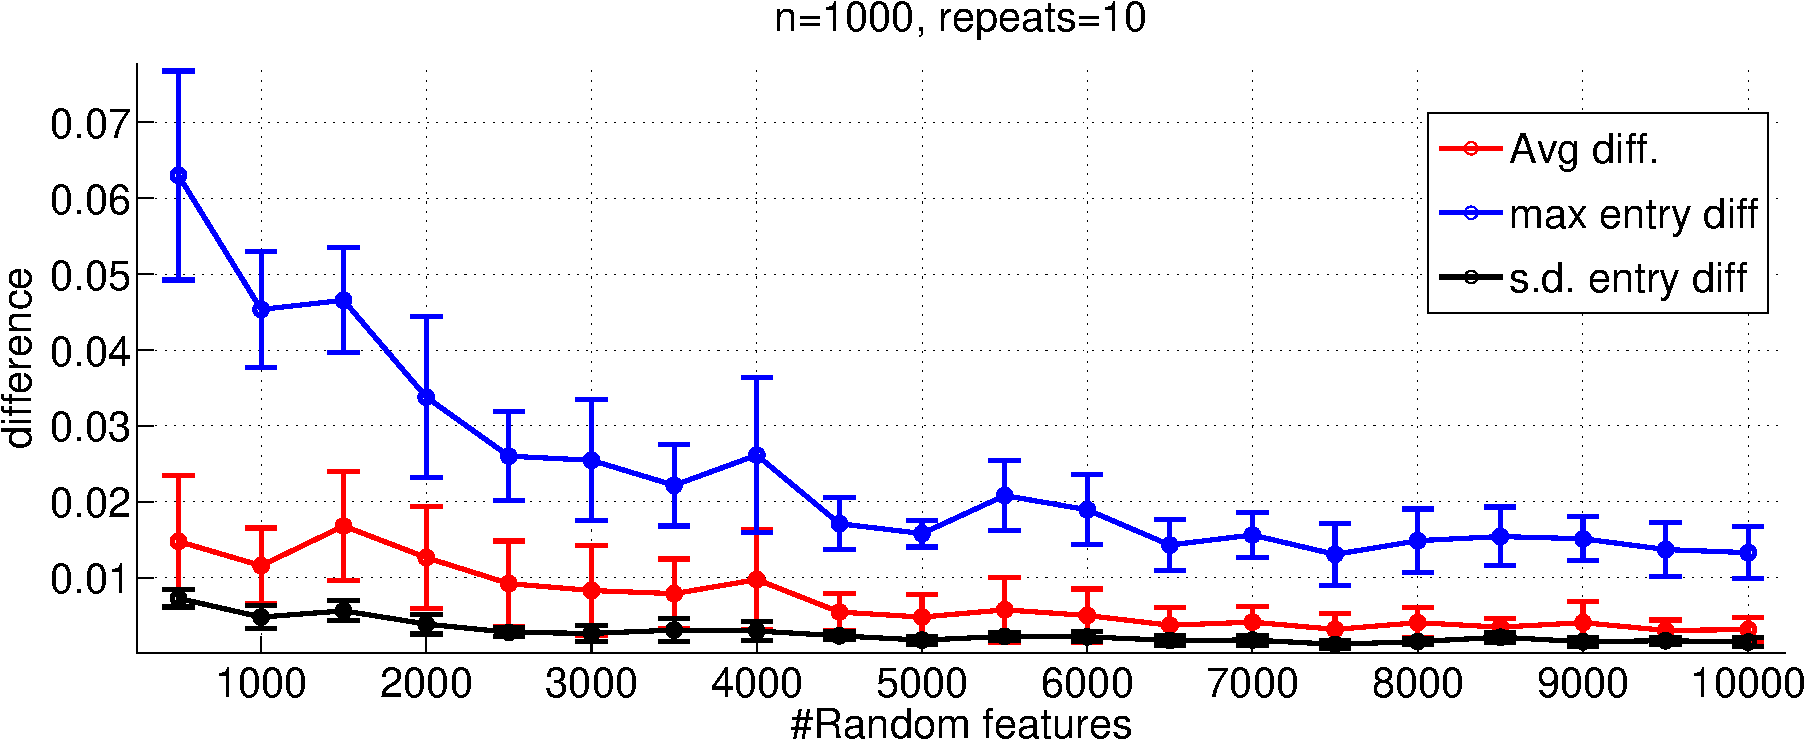
\includegraphics[width=10cm]{img/primal_egauss_sanity-crop}


\subsection{Product Kernel on Mean Embeddings}

The kernel $\kappa$ is defined as a product of kernels on mean embeddings.
For each incoming message $l$, we need one set of random weights
$\{w_{i}^{(l)}\}_{i=1}^{D}\sim\hat{k}^{(l)}$ and $\{b_{i}^{(l)}\}_{i=1}^{D}$.
\begin{align*}
\kappa\left(p,q\right) & =\left\langle \bigotimes_{l=1}^{c}\mu_{p^{(l)}},\bigotimes_{l=1}^{c}\mu_{q^{(l)}}\right\rangle _{\otimes_{l}\mathcal{H}^{(l)}}\\
 & =\prod_{l=1}^{c}\left\langle \mu_{p^{(l)}},\mu_{q^{(l)}}\right\rangle _{\mathcal{H}^{(l)}}\\
 & =\prod_{l=1}^{c}\mathbb{E}_{p^{(l)}(x)}\mathbb{E}_{q^{(l)}(y)}k^{(l)}\left(x-y\right)\\
 & \approx\prod_{l=1}^{c}\hat{\phi}^{(l)}(p^{(l)})^{\top}\hat{\phi}^{(l)}(q^{(l)})\\
 & =\hat{\varphi}(p)^{\top}\hat{\varphi}(q)
\end{align*}
where $\hat{\varphi}(p):=\left(\hat{\phi}_{i_{1}}^{(1)}\times\cdots\hat{\phi}_{i_{c}}^{(c)}\right)_{i_{1}\cdots i_{c}=1}^{c}=\hat{\phi}^{(1)}\circledast\hat{\phi}^{(2)}\circledast\cdots\circledast\hat{\phi}^{(c)}\in\mathbb{R}^{D^{c}}$.
The symbol $\circledast$ denotes a Kronecker product and we assume
that each $\hat{\phi}^{(l)}\in\mathbb{R}^{D}$. Without a special
solver which can take advantage of the Kronecker product in $\hat{\varphi}$,
this random feature map might be impractical due to large memory requirement
unless $D$ is very small. 


\subsection{Sum Kernel on Mean Embeddings}

If we instead define $\kappa$ as the sum of $c$ kernels, we have
\begin{align*}
\kappa(p,q) & =\sum_{l=1}^{c}\left\langle \mu_{p^{(l)}},\mu_{q^{(l)}}\right\rangle _{\mathcal{H}^{(l)}}\\
 & \approx\sum_{l=1}^{c}\hat{\phi}^{(l)}(p^{(l)})^{\top}\hat{\phi}^{(l)}(q^{(l)})\\
 & =\hat{\varphi}(p)^{\top}\hat{\varphi}(q)
\end{align*}
where $\hat{\varphi}(p):=\left(\hat{\phi}^{(1)}(p^{(1)})^{\top},\ldots,\hat{\phi}^{(c)}(p^{(c)})^{\top}\right)^{\top}\in\mathbb{R}^{cD}$
whose memory requirement is much lower.




\subsubsection{Kernel on tuples of messages}

As our prediction is from $M_{j}=[m_{V_{i}\rightarrow f}^{j}(v_{i})]_{i=1}^{c}$
($c$ is the number of variables connected to the factor $f$) to
$y_{j}$, in the end, the kernel we need is $\kappa(M_{i},M_{j})$
which is defined on message tuples.
\begin{align*}
\kappa\left(M_{i},M_{j}\right) & =\prod_{l=1}^{c}\kappa_{l}\left(m_{V_{l}\rightarrow f}^{i},m_{V_{l}\rightarrow f}^{j}\right)
\end{align*}
which is a product of Gaussian kernels on mean embedding of each message.
With random features, we have 
\[
\kappa(M_{i},M_{j})\approx\prod_{l=1}^{c}\hat{\psi}_{l}(p_{l}^{i})^{\top}\hat{\psi}_{l}(p_{l}^{j})=\hat{\Psi}(M_{i})^{\top}\hat{\Psi}(M_{j})
\]
where $\hat{\Psi}(M_{i}):=\left(\left(\hat{\psi}_{1}(p_{1}^{i})_{i_{1}}\right)\times\cdots\times\left(\hat{\psi}_{c}(p_{c}^{i})_{i_{c}}\right)\right)_{i_{1}\cdots i_{c}=1}^{c}=\hat{\psi}_{1}(p_{1}^{i})\circledast\hat{\psi}_{2}(p_{2}^{i})\circledast\cdots\circledast\hat{\psi}_{c}(p_{c}^{i})\in\mathbb{R}^{D_{out}^{c}}$.
The symbol $\circledast$ denotes a Kronecker product. The total number
of random features is given by $D=\left(D_{out}\right)^{c}$. It can
be seen that the total number of features grows exponentially in the
number of connected variables. We can also use 
\begin{align*}
\kappa\left(M_{i},M_{j}\right) & =\sum_{l=1}^{c}\kappa_{l}\left(m_{V_{l}\rightarrow f}^{i},m_{V_{l}\rightarrow f}^{j}\right)
\end{align*}
which gives $D=cD_{out}$. We expect the product kernel to be able
to better capture the interaction among incoming messages.

Yet another way to form a kernel on tuples of messages is to consider
a joint embedding. Let $\mathbb{M}_{i}:=\prod_{l=1}^{c}m_{V_{l}\rightarrow f}^{i}(v_{l})$
e.g., a product of all incoming messages. We can treat $\mathbb{M}_{i}$
as a joint distribution of one variable $V:=(v_{1},\ldots,v_{c})$.
A joint embedding kernel is straightforwardly given by defining a
Gaussian kernel on mean embeddings of these joint distributions:
\[
\kappa(M_{i},M_{j})=\kappa_{\text{gauss}}(\mathbb{M}_{i},\mathbb{M}_{j}).
\]
An advantage of this kernel is that the final number of random features
is $D_{out}$ as compared to $D_{out}^{c}$ (product kernel) and $cD_{out}$
(sum kernel). One potential disadvantage is that we treat all neighbouring
variables as independent.


\paragraph{Experiments on Random Features for Gaussian Kernel on Mean Embeddings }

It is unclear how $D_{in}$ and $D_{out}$ affect the quality of the
random feature approximation. We quantify the effect empirically as
follows. We generate 300 Gaussian messages, compute the true gram
matrix and the approximate gram matrix given by the random features,
and report the Frobenius norm of the difference of the two matrices
on a grid of $D_{in}$ and $D_{out}$. For each $(D_{in},D_{out})$,
we repeat 20 times with a different set of random features and report
the averaged Frobenius norm.

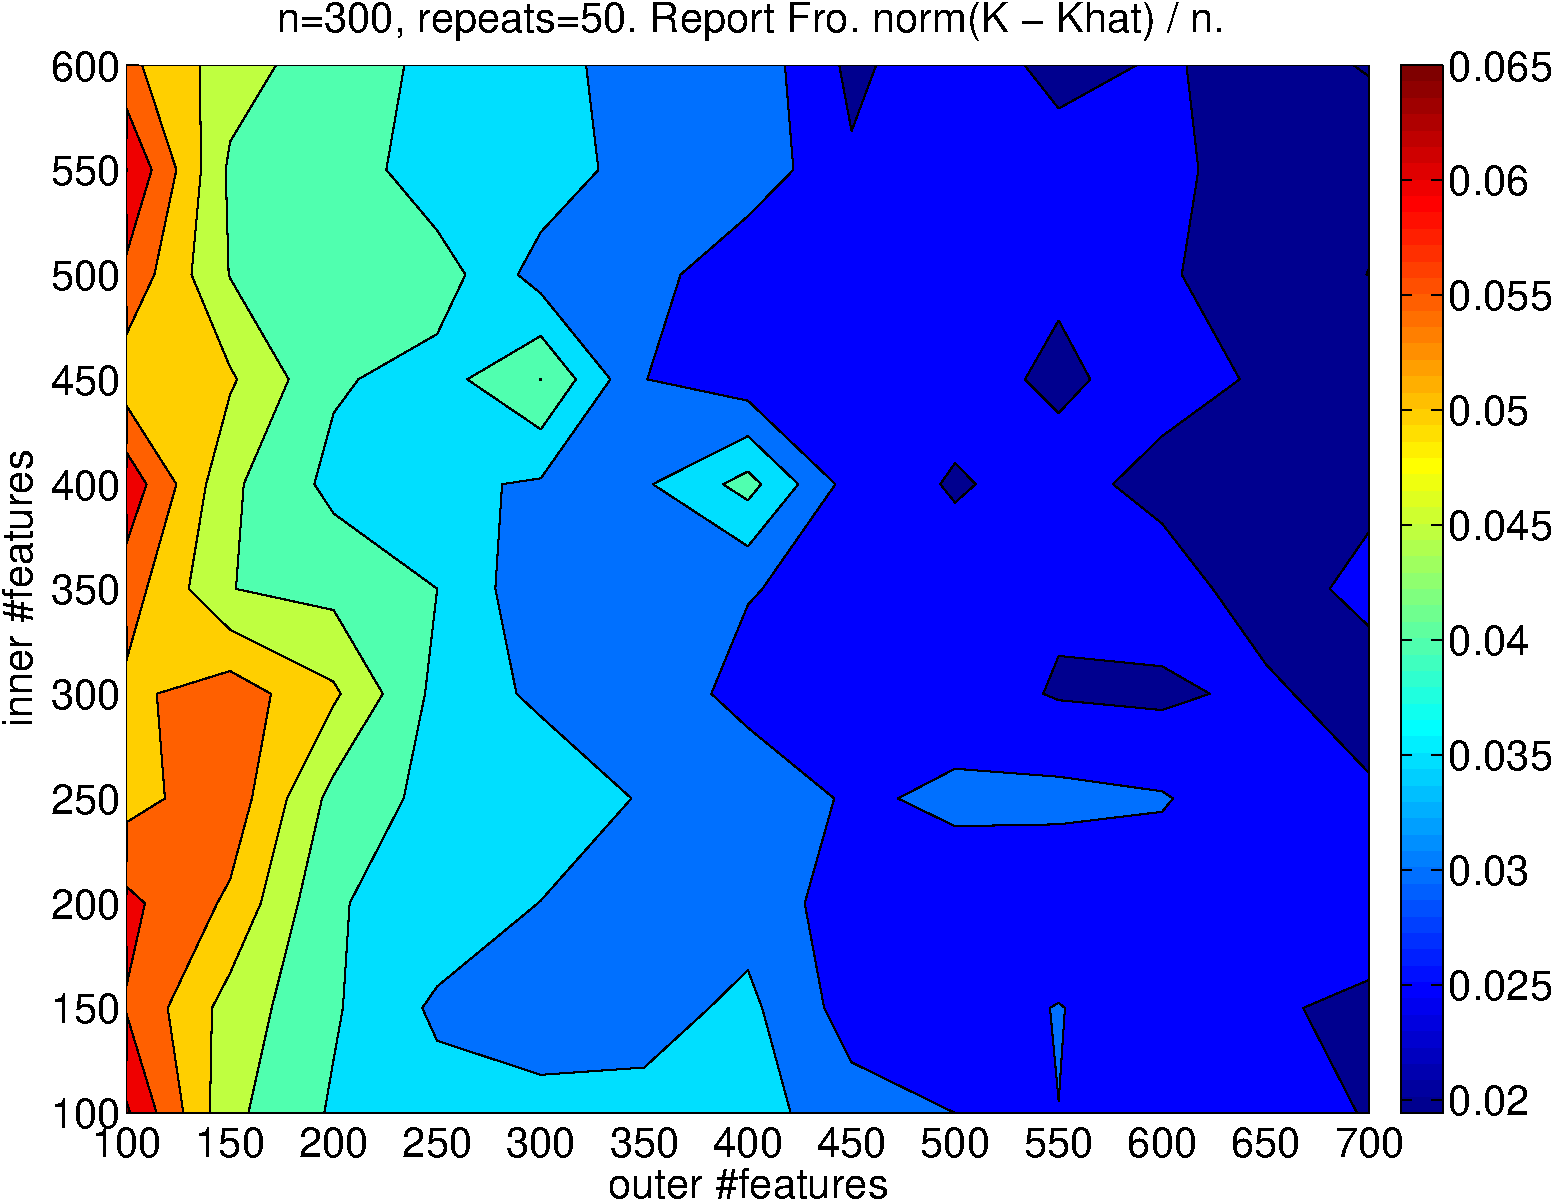
\includegraphics[width=8cm]{img/kggauss_rf_grid-crop} 

The result suggests that $D_{out}$ has more effect in improving the
approximation.


\bibliographystylesup{abbrvnat}
\bibliographysup{refappendix} 
\end{document}
